\section{Rigid Bodies: Fluid-Structure Interaction}
\label{sec:FB_validation}

Section \ref{sec:NS_validation} introduced some validations of the proposed \ac{SPH} method, exclusively dealing with fixed, or with otherwise imposed motion, solid boundaries. In this Section, boundaries with \ac{DOF}s are studied. As described in Chapter \ref{cap:int}, the fluid and rigid body problem within \ac{SPH} discretizations has been treated previously and validations have been presented. The next Sections focus on the comparison of buoyancy and fluid-structure interaction with available solutions. Numerical stability and qualities of the implementation are also addressed in idealized cases.

Due to insufficient solutions and data on complex, multi-body free surface fluid-structure interactions, an extensive experimental campaign was designed and carried out, as explored in Section \ref{sec:validation_exp}.


\subsection{Free stream consistency}
\label{Subsect:free_stream}
%
A simple property of a discretization method should be free stream compliance. For a given velocity of the fluid and the rigid body, given that initial relative velocities are zero, they should remain zero as time evolves and the equations are integrated, showing that there are no errors in the integrators and that these are robust regarding truncation errors. The first case consists of a $6 \times 6 \times 6$ m patch of fluid and a $2 \times 2 \times 2$ m rigid square in the center of the fluid, with a $Dp=0.05$ m initial inter particle spacing, equal in all three dimensions. Both are given a $u=1\text{ ms}^{-1}$ initial velocity, gravity acceleration is zero and there are no other solid boundaries. Figure \ref{fig:Free_stream_C1} shows a bidimensional slice of the velocity field, around the lower right corner of the rigid square.
%
\begin{figure}[ht!]
	\centering
	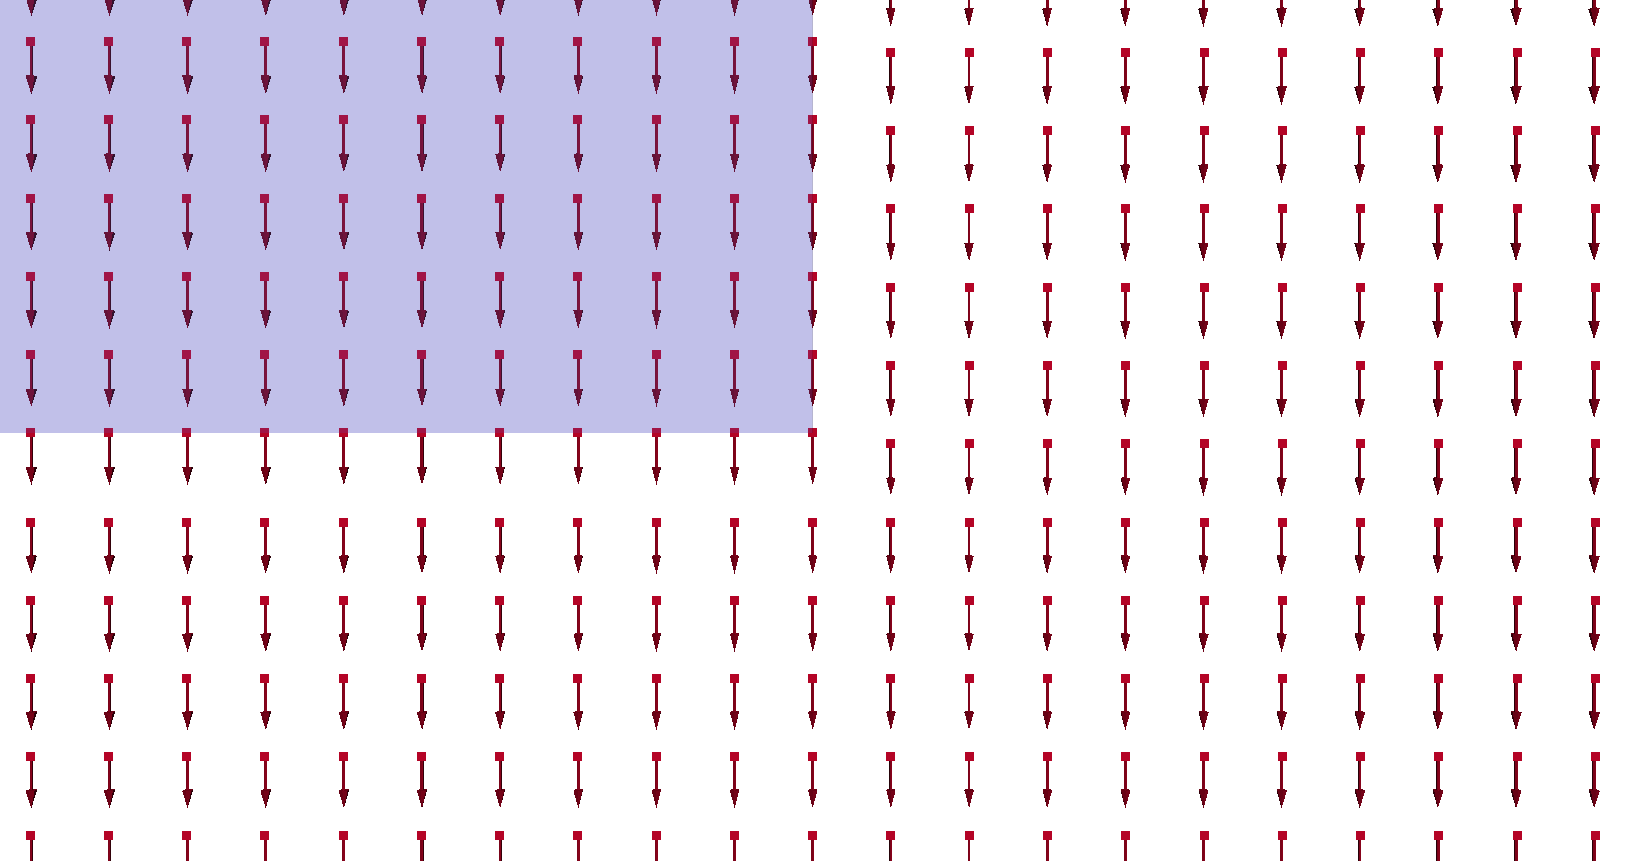
\includegraphics[width=0.5\linewidth]{Figures/5.Chapter/fig1}
	\caption{Velocity field detail for a corner of the square at any time step.}
	\label{fig:Free_stream_C1} 
\end{figure}
%

The field is constant in time, no deviations along the solid-fluid interface were introduced during the $30\;s$ of simulation. 

A more demanding case is to consider a non-zero acceleration, since numerical errors arising from the usage of two sets of equations (for fluid and rigid bodies) should be more noticeable. The same geometry as for the previous example is set up, but with zero initial velocity and non-zero constant acceleration. Figure \ref{fig:Free_stream_C2} shows a slice of the velocity fields at three separate instants.
%
\begin{figure}[ht!]
	\centering
	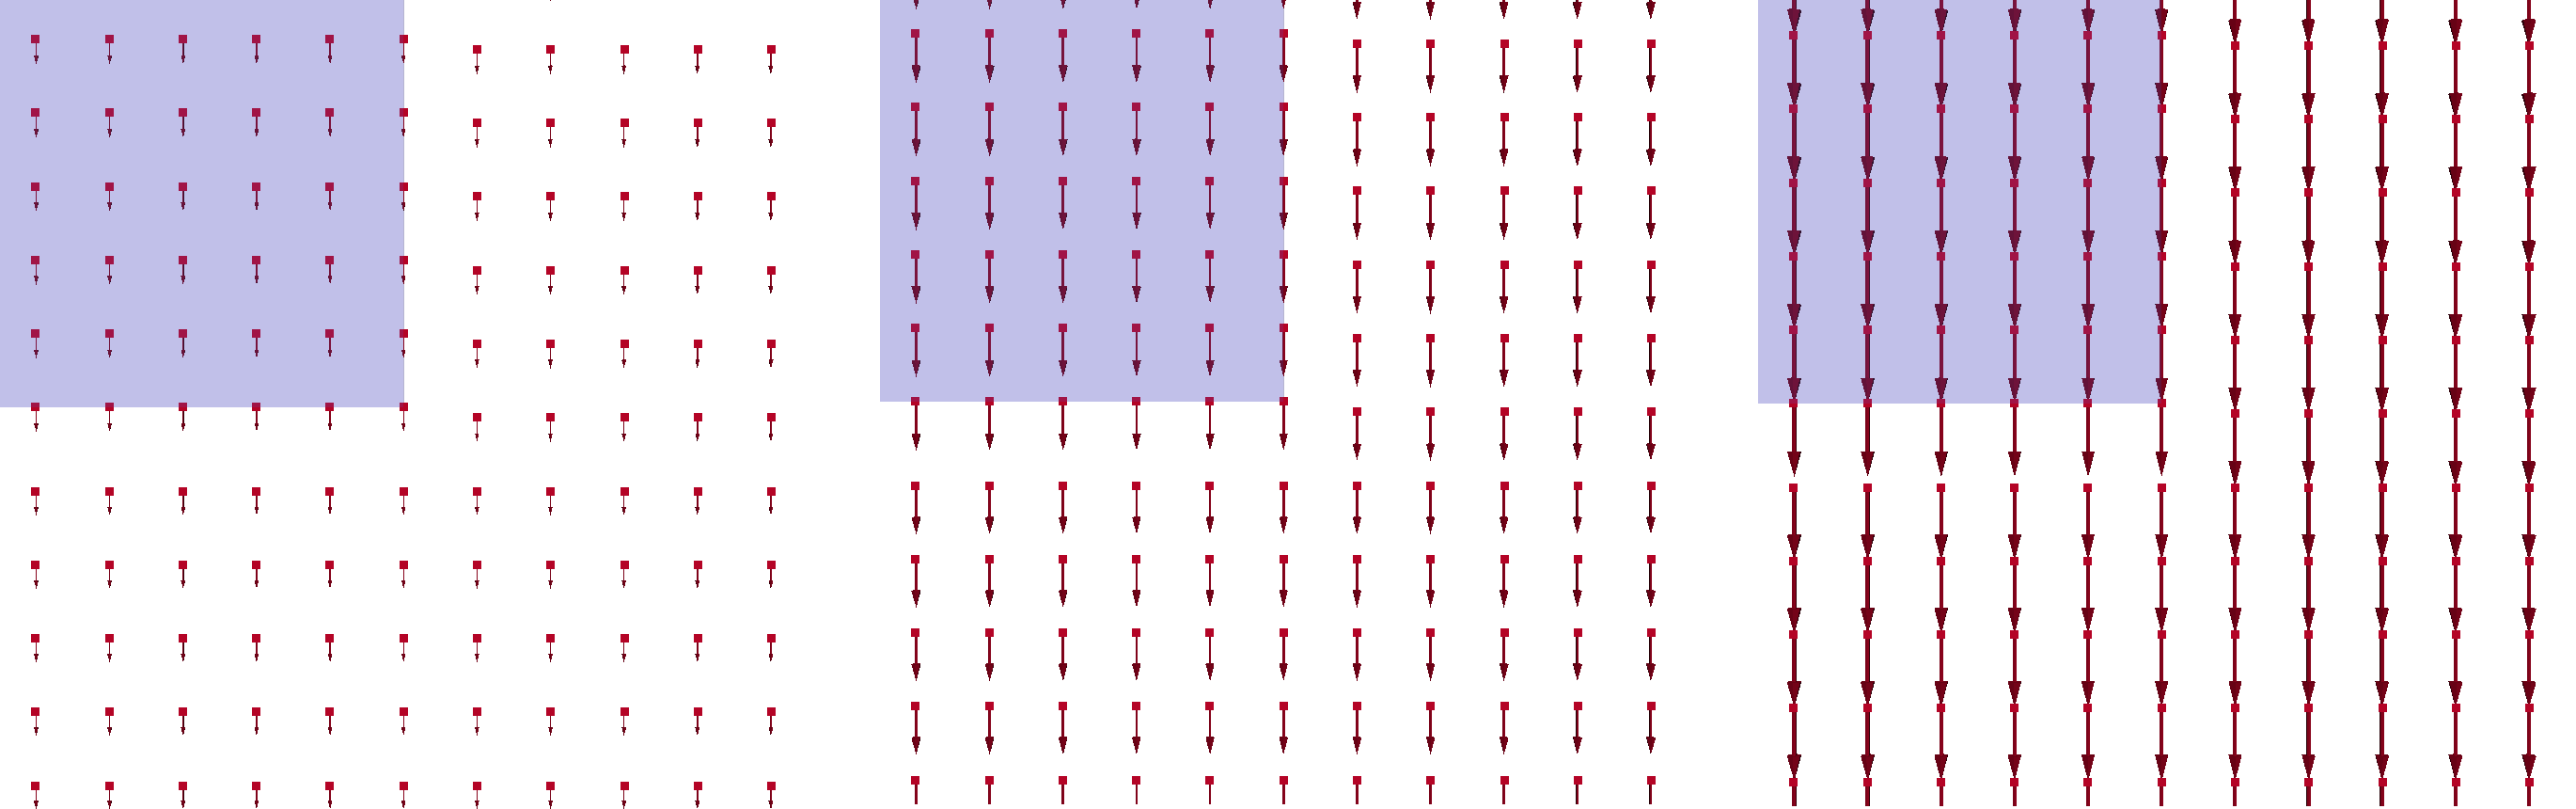
\includegraphics[width=0.9\linewidth]{Figures/5.Chapter/fig2_I}
	\caption{Velocity field detail for a corner of the square at $t=5s$, $t=10s$ and $t=15s$.}
	\label{fig:Free_stream_C2} 
\end{figure}
%

The error of the object velocity comparing to the overall field is neglectable in the first two snapshots and reaches $0.13\%$ for third one. The same conclusions as for the first case can be drawn: the velocity field evolves without irregularities being developed at the fluid-solid interface, streamlines are virtually not disturbed by numerical errors.


%%%%%%%%%%%%%%%%%%%%%%%%%%%%%%%%%%%%%%%%%%%%%%%%%%%%%%%%%%%%%%%%%
\subsection{Buoyancy and Fluid/Solid Interfaces}
\label{sec:validation_buoyancy}

\subsubsection{Fluid/Solid Interfaces}
\label{sec:Fluid/Solid Interfaces}

The interface between fluid and solid particles is subjected to similar deficiencies as described for large density ratio cases \cite{Colagrossi-2003}, in this case generated by forcing the relative position of the solid phase particles. An overestimation of the density on the solid particles occurs, producing a hydrophobic effect that results in a reorganization of the fluid particle positions. This happens in order to cope with the increased density gradient at the interface and the entropy jump that occurs, considering that the solid particles are ordered strictly, not necessarily generating a constant equilibrium distance for a fluid particle across the interface. The $\delta$-SPH term prescribed in expressions \eqref{eq:sph_navier_cont_delta_sph} and \eqref{eq:delta_sph_molteni} effectively curb these cascade behaviors by not allowing an erroneous density field to be computed at the interface locus. Figure \ref{fig:delta_posits} illustrates the difference in particle distribution with and without the $\delta$-SPH term across a fluid-solid interface of a cylinder with $r=1$ m.
%
\begin{figure}[ht!]
	\centering
	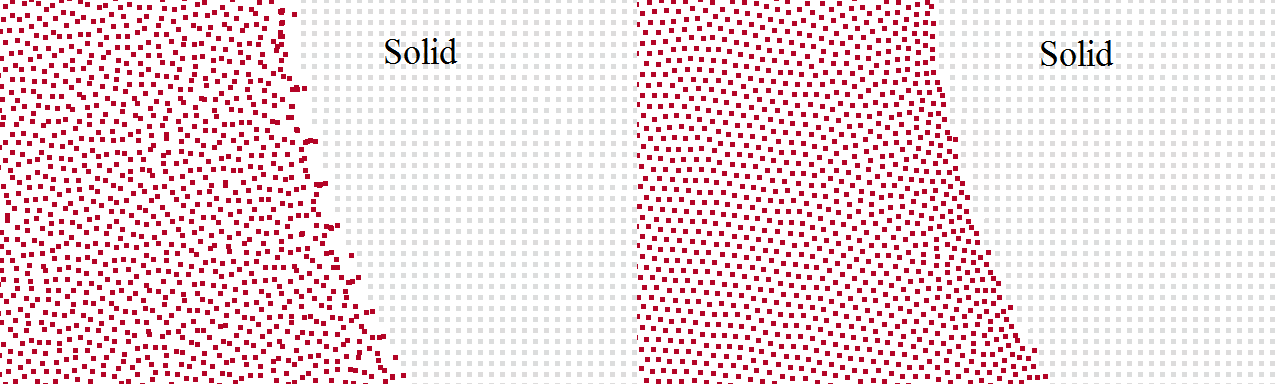
\includegraphics[width=0.8\linewidth]{Figures/5.Chapter/fig1b_text}
	\caption{Fluid-solid interface. Left $\delta=0$, right $\delta=0.1$ }
	\label{fig:delta_posits} 
\end{figure}
%

Figure \ref{fig:delta_dens} shows the density profiles in a normal direction to the interface.
%
\begin{figure}[ht!]
	\centering
	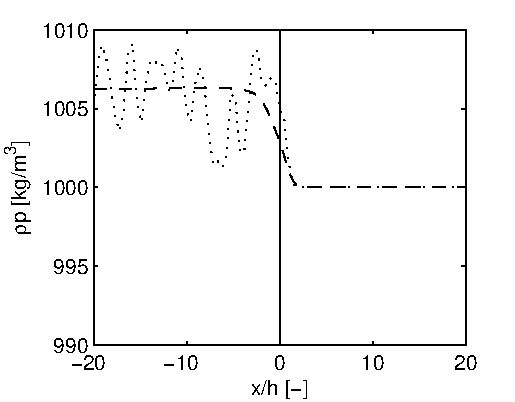
\includegraphics[width=0.45\linewidth]{Figures/5.Chapter/fig2a} 
	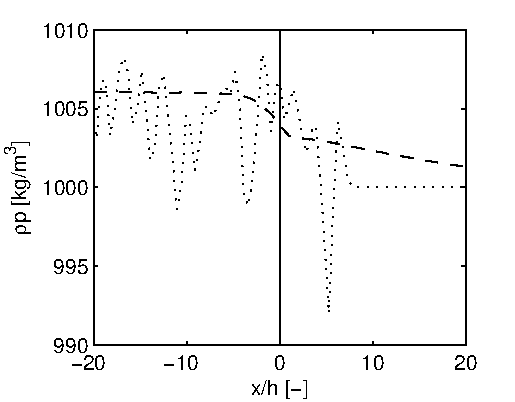
\includegraphics[width=0.45\linewidth]{Figures/5.Chapter/fig3a}
	\caption{Density profiles for $t=10$ s. Left, non-mobile boundary, right, mobile boundary. Interface position (---), $\delta$=0 ($\cdots$), $\delta$=0.1 (-- -- --)}
	\label{fig:delta_dens} 
\end{figure}
%
The profiles show the density fluctuations around the interface for a static and a moving boundary. The moving boundary was created by moving the cylinder at $v=0.1$ m/s. On the fluid region one can see a large density overestimation in both cases, causing the particles to rearrange as in figure \ref{fig:delta_posits}, in accordance with the findings of \cite{Saitoh-2013}. With a non-zero $\delta$ the density profile is smooth and no fluctuations are detected, enabling the fluid particles to remain at similar distance from the solid and other fluid particles. The kernel should now present a more uniform stencil, providing more accurate interpolations.

%%%%%%%%%%%%%%%%%%%%%%%%%%%%%%%%%%%%%%%%%%%%%%%%%%%%%%%%%%%%%%%%%%%%%%%%
\subsubsection{Buoyancy: analytical and numerical solutions}
\label{subsec:boyant_analytical}

Since the interface description seems to perform as expected, the traditional way to verify the integrity of the terms is by analyzing the buoyancy driven motion of bodies in a fluid. The used configuration consists of a cylinder, whose density is different from that of the fluid, initially placed at a specific depth in a viscous fluid. Both fluid and solid body are initially at rest. Once the motion is initiated, the rate of change of cylinder momentum is, for large values of cylinder Reynolds number ($Re_p$), essentially a function of: i) the body forces associated to the virtual added mass, ii) the Basset history\footnote{Many times neglected, this term represents the temporal delay in boundary layer development as the relative velocity changes with time \citep{Crowe-1998}.}, iii) the buoyancy, iv) the surface forces associated to the gradient of hydrodynamic variables, of which the pressure gradient (buoyancy not included) is the dominant term, and v) viscous drag \cite{Crowe-1998}. The latter, for large $Re_p$ depends on the square of the relative velocity and on a drag coefficient which is approximately $1$ in the range $Re_p = 1\times 10^4$ to $3\times 10^5$.

\cite{Moyo-2000} studied this problem using an inviscid flow model that included only the effects of buoyancy, of the virtual added mass and the pressure gradient. \cite{Fekken-2004} later compared these results with those of another inviscid solution including only added mass and buoyancy and with those of a numerical model based on a \ac{VOF} discretization technique. The latter provides the most relevant comparison, since viscous stresses for the fluid and drag forces on the cylinder are considered and the \ac{VOF} method explicitly tracks free surface geometry changes without any special treatment, unlike the solution of \cite{Moyo-2000}. 

The simulations reproduce the conditions described in \cite{Fekken-2004}: cylinders with a $r=1m$ radius and densities $\rho=0.6\rho_{w}$ and $\rho=0.9\rho_{w}$ are placed at a depth of $D=5$ m, measured from the free-surface to the centroid of the cylinder. The 2D simulation has a domain of an $8m$ long periodic box with a fluid depth of $7m$ and a rigid boundary at the bottom. The initial inter particle spacing are $D/Dp=66$, $D/Dp=100$ and $D/Dp=150$. Cylinder velocities are computed at the centroid of the cylinder and are non-dimensionalised as $V=u/\sqrt{gr}$, were $u$ is the velocity and $g$ is the acceleration of gravity. Time is made non-dimensional as $T=t\sqrt{g/r}$.

Figure \ref{fig:311_1_snaps} shows the system for the case $\rho=0.6\rho_{w}$ at four instants and Figure \ref{fig:311_1} shows the velocity of the cylinders for both cases.
%
\begin{figure}[ht!]
	\centering
	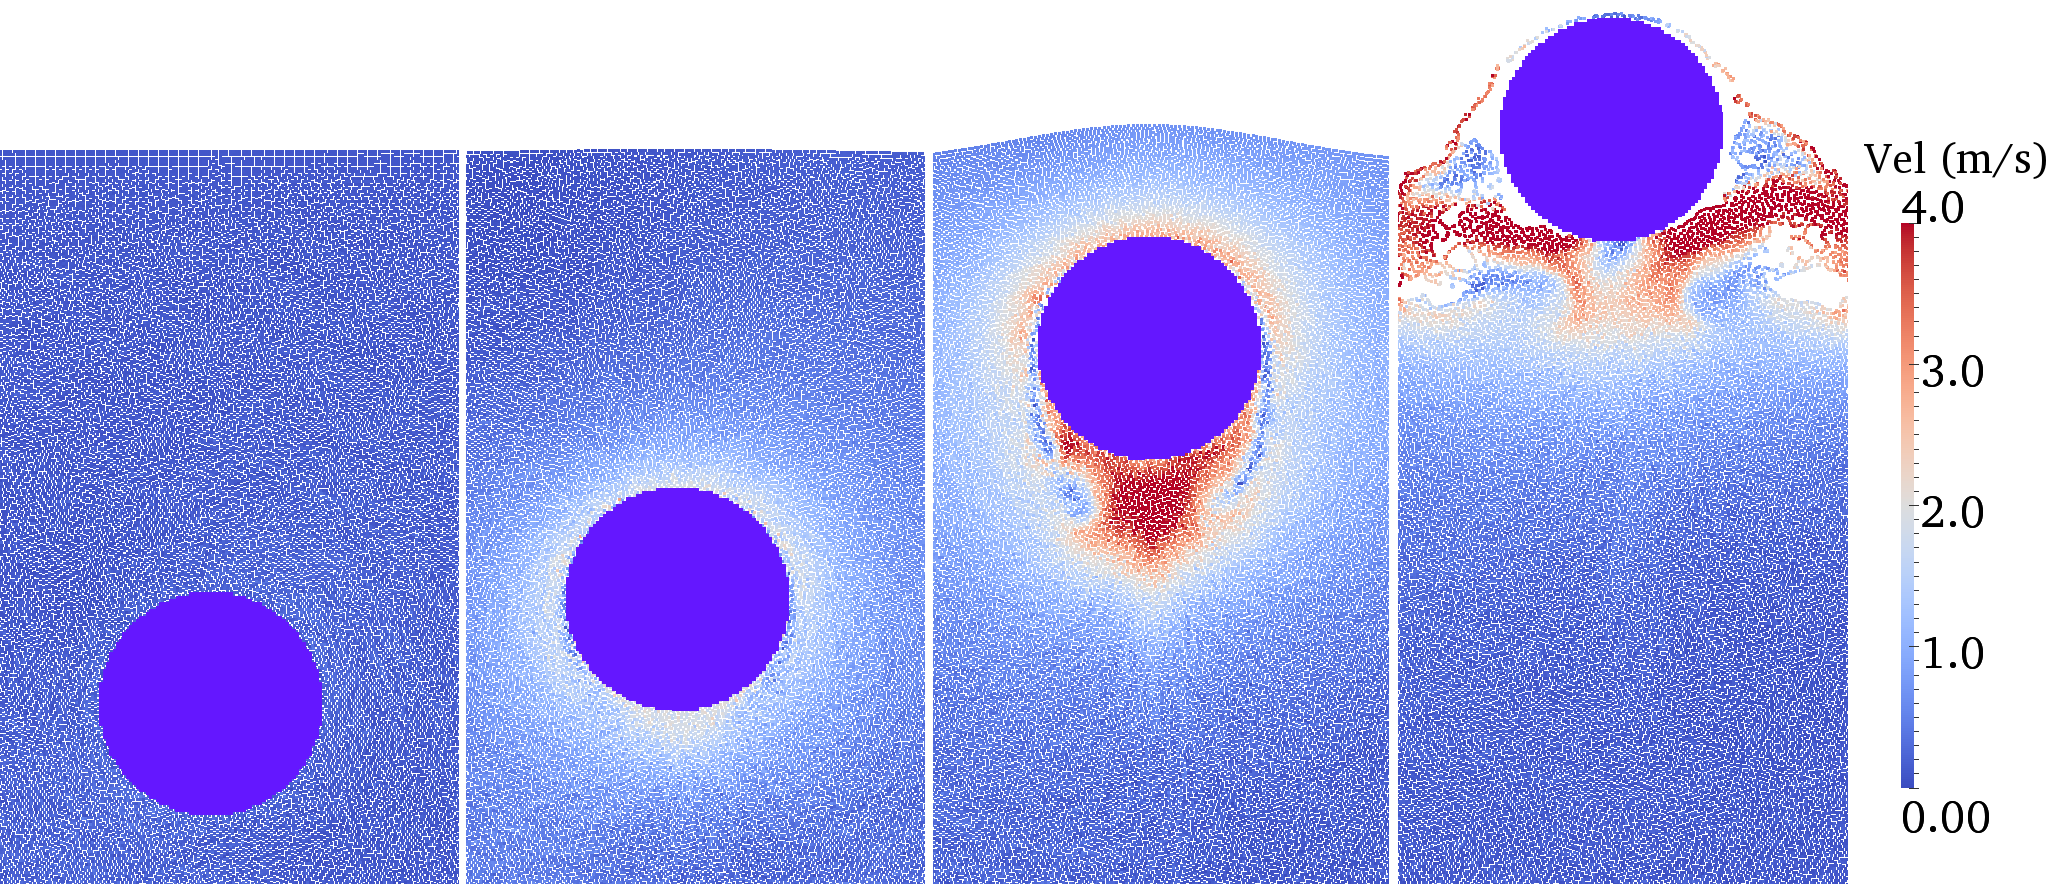
\includegraphics[width=0.9\linewidth]{Figures/5.Chapter/fig5_II} 	
	\caption{{ Rising cylinder with $\rho=0.6\rho_{w}$. $T=0$; $T=3.13$; $T=6.26$; $T=9.40$.}}
	\label{fig:311_1_snaps} 
\end{figure}
%

%
\begin{figure}[ht!]
	\centering
	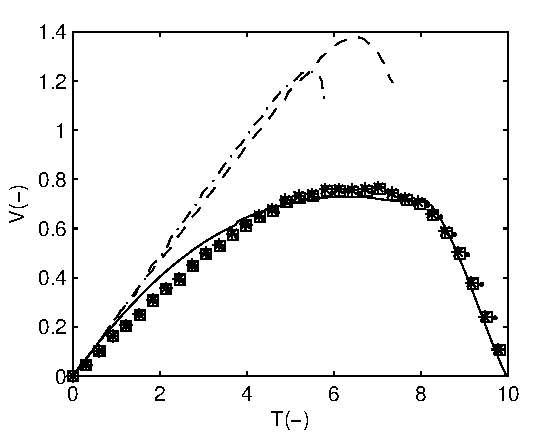
\includegraphics[width=0.49\linewidth]{Figures/5.Chapter/fig10} 
	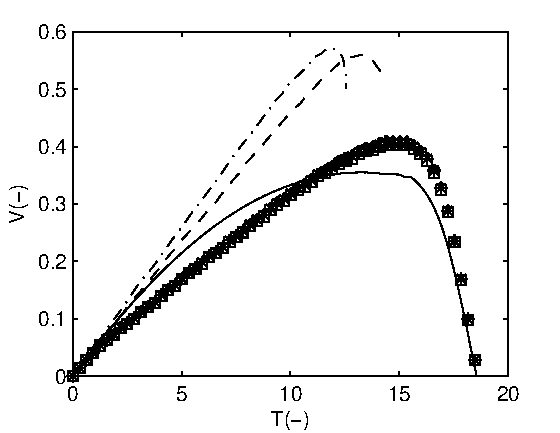
\includegraphics[width=0.49\linewidth]{Figures/5.Chapter/fig11}
	\caption{{Non-dimensional vertical velocity for a cylinder. Left - $\rho=0.6\rho_{w}$; Right - $\rho=0.9\rho_{w}$. Added mass model(analytical)\cite{Fekken-2004}($-\cdot-$); Moyo \& Greenhow(analytical)\cite{Moyo-2000}($---$); Fekken(\ac{VOF})\cite{Fekken-2004}($-$); DualSPHysics $D/Dp=66$($\bullet$), $D/Dp=100$($\ast$) and $D/Dp=150$($\Box$).}}
	\label{fig:311_1} 
\end{figure}
%

The value $Re_p$ is larger than $1 \times 10^{4}$ for cylinder velocities larger than $1 \ \mathrm{cm s^{-1}}$, which is equivalent to $V > 0.003$. Also, $Re_p = 3 \times 10^{5}$ is attained at $V = 0.096$. Phenomenologically, and in what concerns the drag force, it is expected that between $V = 0.003$ and $V=0.096$ the separation point of the laminar boundary layer attached to the cylinder remains stable and, as a consequence, $Re_p$ effects are negligible, with the value of the drag coefficient remaining close to $1$. At approximately $V=0.096$ the boundary layer becomes turbulent, the separation point progresses considerably and the drag coefficient is reduced. From this point onwards the drag coefficient becomes a mild increasing function of $Re_p$. Basset forces should become relevant only near the free-surface, when the cylinder decelerates. Near the free-surface virtual added mass and pressure gradients vary non-linearly with the overall effect of reduction the cylinder acceleration to the point of becoming negative \citep{frank-1967}.

Observing the results shown in Figure \ref{fig:311_1} one notes that the inviscid models of \cite{Moyo-2000} and \cite{Fekken-2004} show a linear evolution of the velocity while the cylinder is far from the free-surface which, given that viscous terms are absent, indicates that both added mass and pressure gradients remain approximately constant in this reach. Closer to the free-surface, their models feature the expected reduction of cylinder acceleration. The \ac{VOF} model of \cite{Fekken-2004} agrees with the inviscid models in what concerns the initial acceleration and initial velocity (up to $V = 0.18$ in the $\rho=0.6\rho_{w}$ case and up to $V = 0.1$ in the $\rho=0.9\rho_{w}$ case). The present solutions feature a smaller acceleration, relatively to the inviscid solutions, for $V>0$, in the case of $\rho=0.6\rho_{w}$, and for $V>0.05$, in the case of $\rho=0.9\rho_{w}$. The fact that both \ac{VOF} model of \cite{Fekken-2004} and the present solutions disagree with the inviscid solutions for most of the simulation reach can be attributed to the existence of viscous forces in the former models. The slightly lower velocities observed in the present simulations relatively to the \ac{VOF} solution (for $T<4$ in the $\rho=0.6\rho_{w}$ case and $T<10$ in the $\rho=0.9\rho_{w}$ case) can be due to the different discretization techniques and numerical approaches for fluid-solid interaction.

The effects of the changes in the nature of the cylinder boundary layer are not immediately visible in the \ac{VOF} solution of \cite{Fekken-2004} and in the present solutions. Indeed, Figure \ref{fig:311_1} shows that there are no apparent discontinuities in the slope of the \ac{VOF} solutions. The present simulations do show a change in acceleration at $V=0.1$, for the $\rho=0.6\rho_{w}$ case, and at $V=0.07$, for the $\rho=0.9\rho_{w}$ case. However, it is not obvious if this is related to the breakdown of the laminar boundary layer (that should occur at $V=0.096$) since, in both cases, there is a local reduction of acceleration while the change of boundary layer nature produces a sharp reduction of the drag coefficient. One hints that both the \ac{VOF} solution of \cite{Fekken-2004} and the present solutions feature an insufficient resolution of the boundary layer. A detailed investigation of the behavior of cylinder boundary layer was not presented by \cite{Fekken-2004} and, in the case of the present simulations, is out of the scope of this work. Present solutions and \ac{VOF} solution of \cite{Fekken-2004} differ also in the value of the acceleration in the intermediate reaches. This is most visible in the case of $\rho=0.9\rho_{w}$ between $T=2.5$ and $T=10$ (Figure \ref{fig:311_1}) where the present solution features an approximately constant acceleration. The present solutions thus feature an articulation of surface and body forces that render virtually constant the total external force. This is not the case in the \ac{VOF} solution, where the acceleration always decreases. The reasons for this difference are likely to be related to numerical issues, including the treatment of fluid-solid interactions. Differences between the \ac{VOF} and present solutions are also observed when the cylinder approaches the free-surface, but only in the slower case of $\rho=0.9\rho_{w}$: present solutions feature a much faster process of inversion of acceleration signal. As Basset forces may become important when the cylinder approaches the free-surface, one may speculate that fluid-particle interaction may be at the root of the observed differences. Since these differences do not occur in the (faster) $\rho=0.6\rho_{w}$ case, one may also suspect that differences in the treatment of the free-surface between \ac{VOF}-based and \ac{SPH} techniques may be an important component. If that is the case, the faster the approach and thrust through the free-surface, the smaller the differences between both models.

Figure \ref{fig:311_1} also allows to assess the sensitivity of current simulations to numerical resolution. A remarkable aspect of the presented model is that, for both cases, tripling the resolution renders very similar solutions, with slight differences only when the cylinder has already pierced the free-surface. 

%

For a case of engulfment, a cylinder with $\rho=1.2\rho_{w}$ at $D=0$ m (half submerged) is set. Figure \ref{fig:319_6_snaps} shows the state of the system at four instants and Figure \ref{fig:319_6} plots the vertical displacement and velocity of the cylinder.
%
\begin{figure}[ht!]
	\centering
	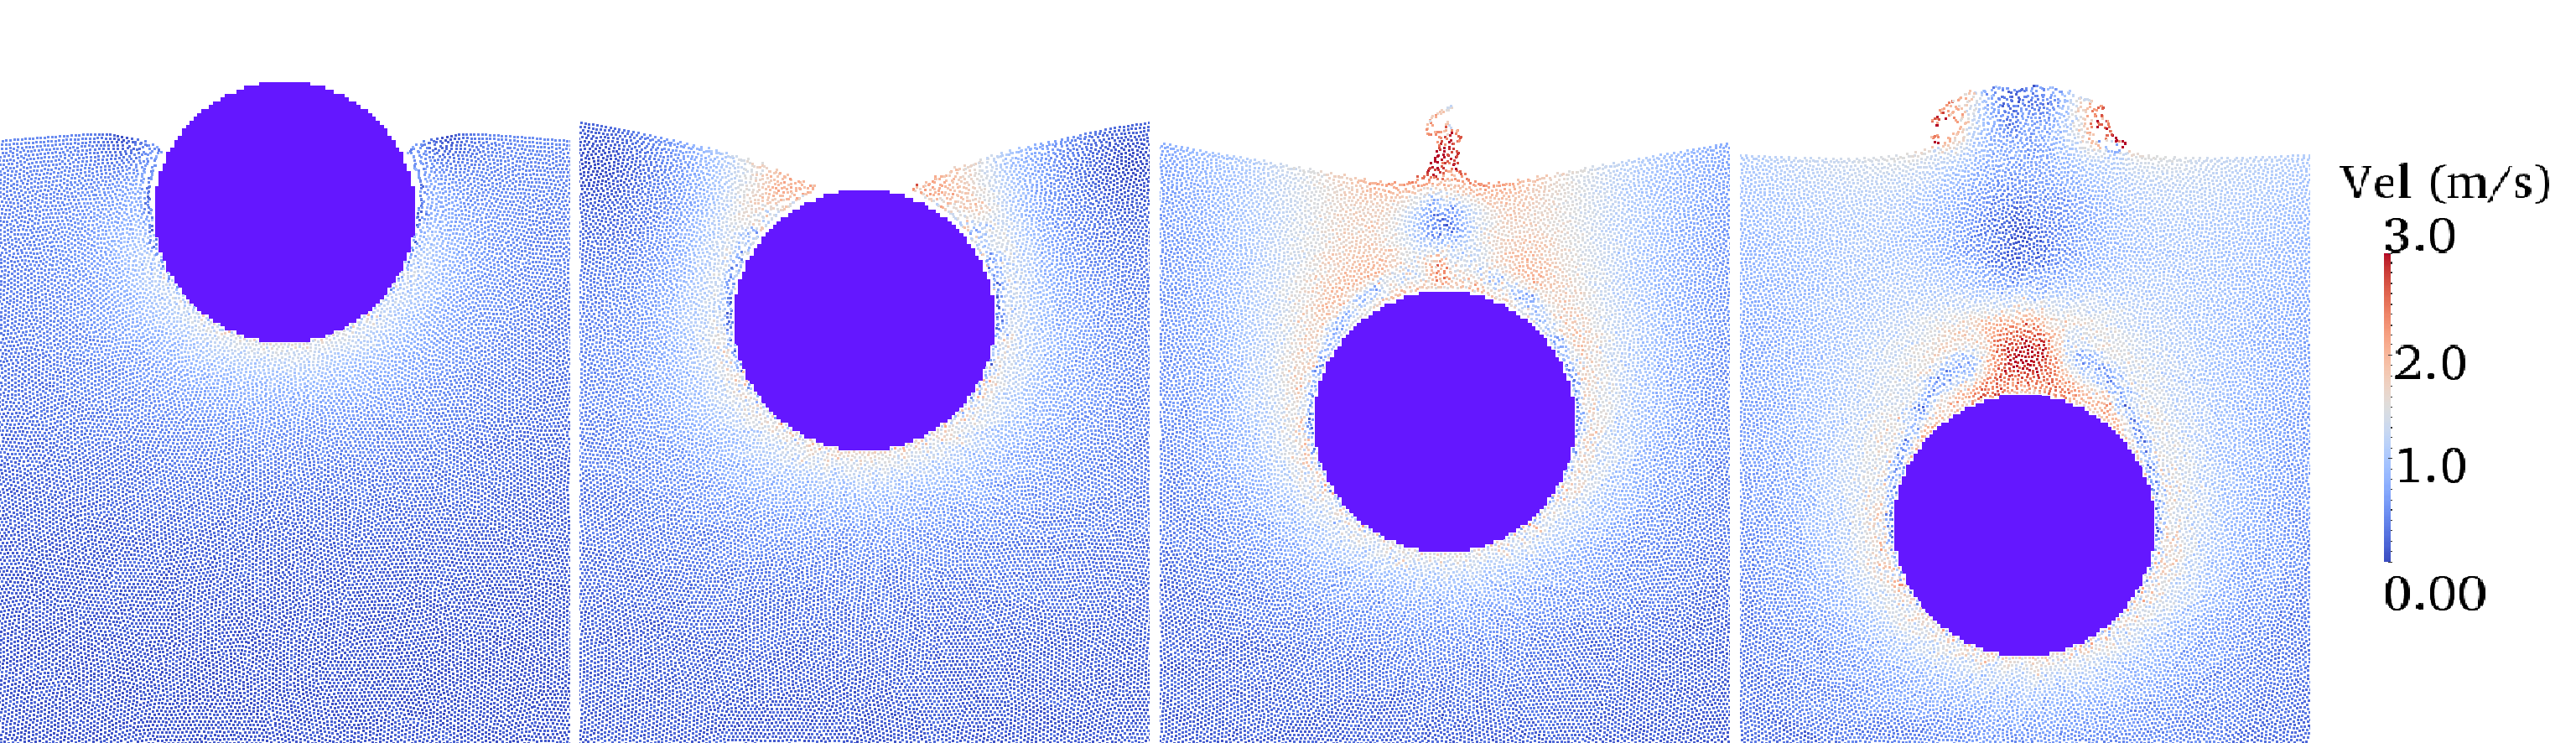
\includegraphics[width=0.9\linewidth]{Figures/5.Chapter/fig12_I}
	%\includegraphics[width=0.2\linewidth]{fig13} 	
	%\includegraphics[width=0.2\linewidth]{fig14}
	%\includegraphics[width=0.2\linewidth]{fig15}
	%\includegraphics[width=0.09\linewidth]{fig16}
	\caption{Sinking cylinder with $\rho=1.2\rho_{w}$. $T=1.57$; $T=3.13$; $T=4.70$; $T=6.27$.}
	\label{fig:319_6_snaps} 
\end{figure}
%
\begin{figure}[ht!]
	\centering
	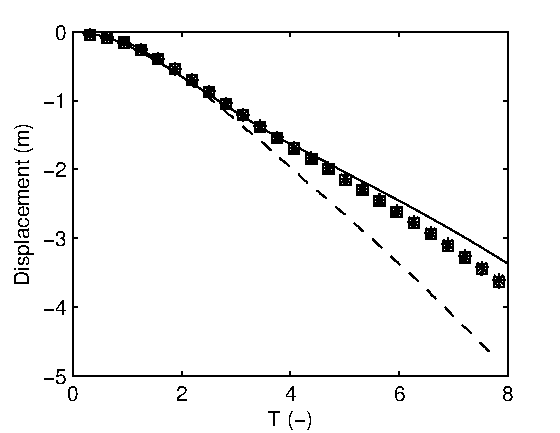
\includegraphics[width=0.45\linewidth]{Figures/5.Chapter/fig17a}
	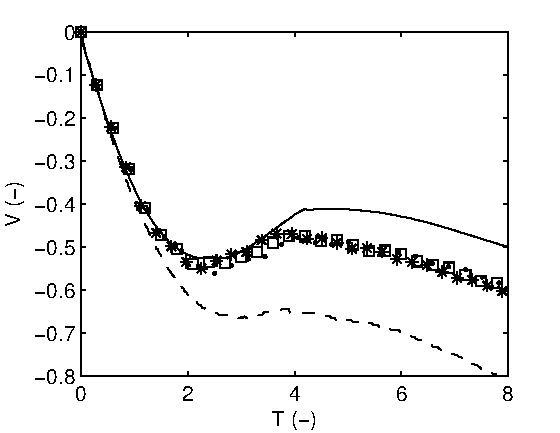
\includegraphics[width=0.45\linewidth]{Figures/5.Chapter/fig18a}
	\caption{{Left - Displacement of cylinder; Right - Non-dimensional vertical velocity for a cylinder of $\rho=1.2\rho_{w}$. Moyo \& Greenhow(analytical)\cite{Moyo-2000}($---$); Fekken(\ac{VOF})\cite{Fekken-2004}($-$); DualSPHysics $D/Dp=66$($\bullet$), $D/Dp=100$($\ast$) and $D/Dp=150$($\Box$).}}
	\label{fig:319_6} 
\end{figure}
%

Again, one can see how the \ac{SPH} results are close to the \ac{VOF} solution, particularly in the initial instants. The inflections on the velocity plots are a result of kinetic energy transfer from the body to the fluid, in order to accommodate the free surface deformations that occurred. At around four time units and for $V\approx-0.5$, the trajectory of the body diverges between the \ac{VOF} and \ac{SPH} solutions. The more resolved tests marginally change the settling velocity on the \ac{SPH} solution.

%%%%%%%%%%%%%%%%%%%%%%%%%%%%%%%%%%%%%%%%%%%%%%%%%%%%%%%%%%%%%%%%%%%%%%%%%%%%%
\subsubsection{Buoyancy: experimental solutions}

Section \ref{subsec:boyant_analytical} introduced analytical upper limits to the velocity evolution of a buoyant sphere and data from numerical experiments from a \ac{VOF} state-of-the-art solution, pointing out some differences to the \ac{SPH} solution. A simple experimental procedure was designed to collect more data and provide yet another comparison point.

Measurements were performed on a glass sphere with $D=0.012$ m, placed over a 0.20 m water column, half submerged. The sphere is kept in place by a suction device and upon its release, an 8-bit $1600\times1200\; \text{px}^2$ CCD camera with a 500 Hz acquisition frame rate records its position until it touches the bottom of the reservoir. The experiment was repeated 3 times in order to provide a notion of repeatability of the apparatus. Three tracking algorithms were employed on each run, based on three image processing routines: edge detection, frame differencing and background subtraction. Three dimensional numerical solutions were performed with $5D$ periodic domain and a rigid bottom. The sphere has $\rho=2.54\rho_{w}$ and two resolutions were tested, $D/Dp=20$ and $D/Dp=50$, resulting in over $50 \times 10^6$ particles for the more resolved case. Figure \ref{fig:exp_glass_figs} offers a comparison between the raw experimental data and the $D/Dp=50$ solution, plotted with the velocity field. 

%
\begin{figure}[ht!]
	\centering
	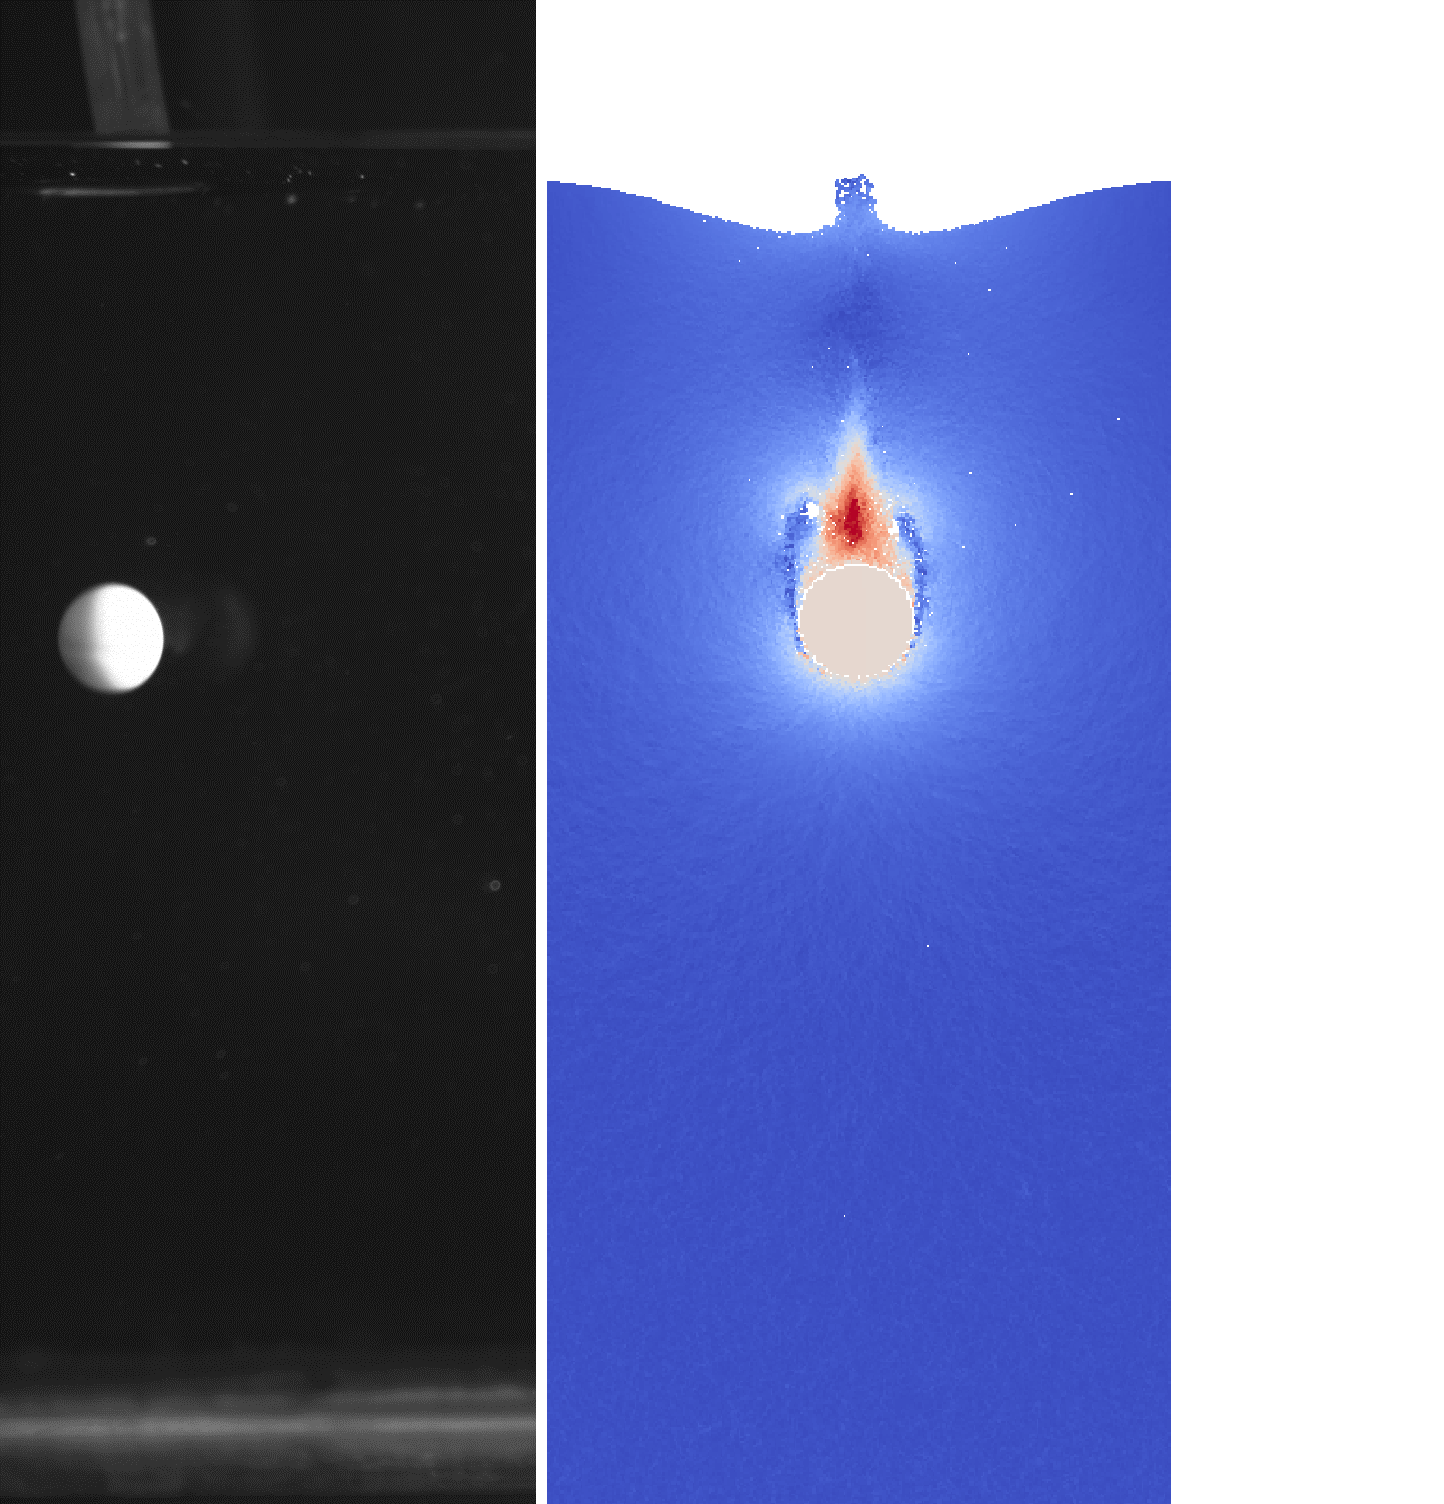
\includegraphics[width=0.48\linewidth]{Figures/5.Chapter/86-6_95_cut}
	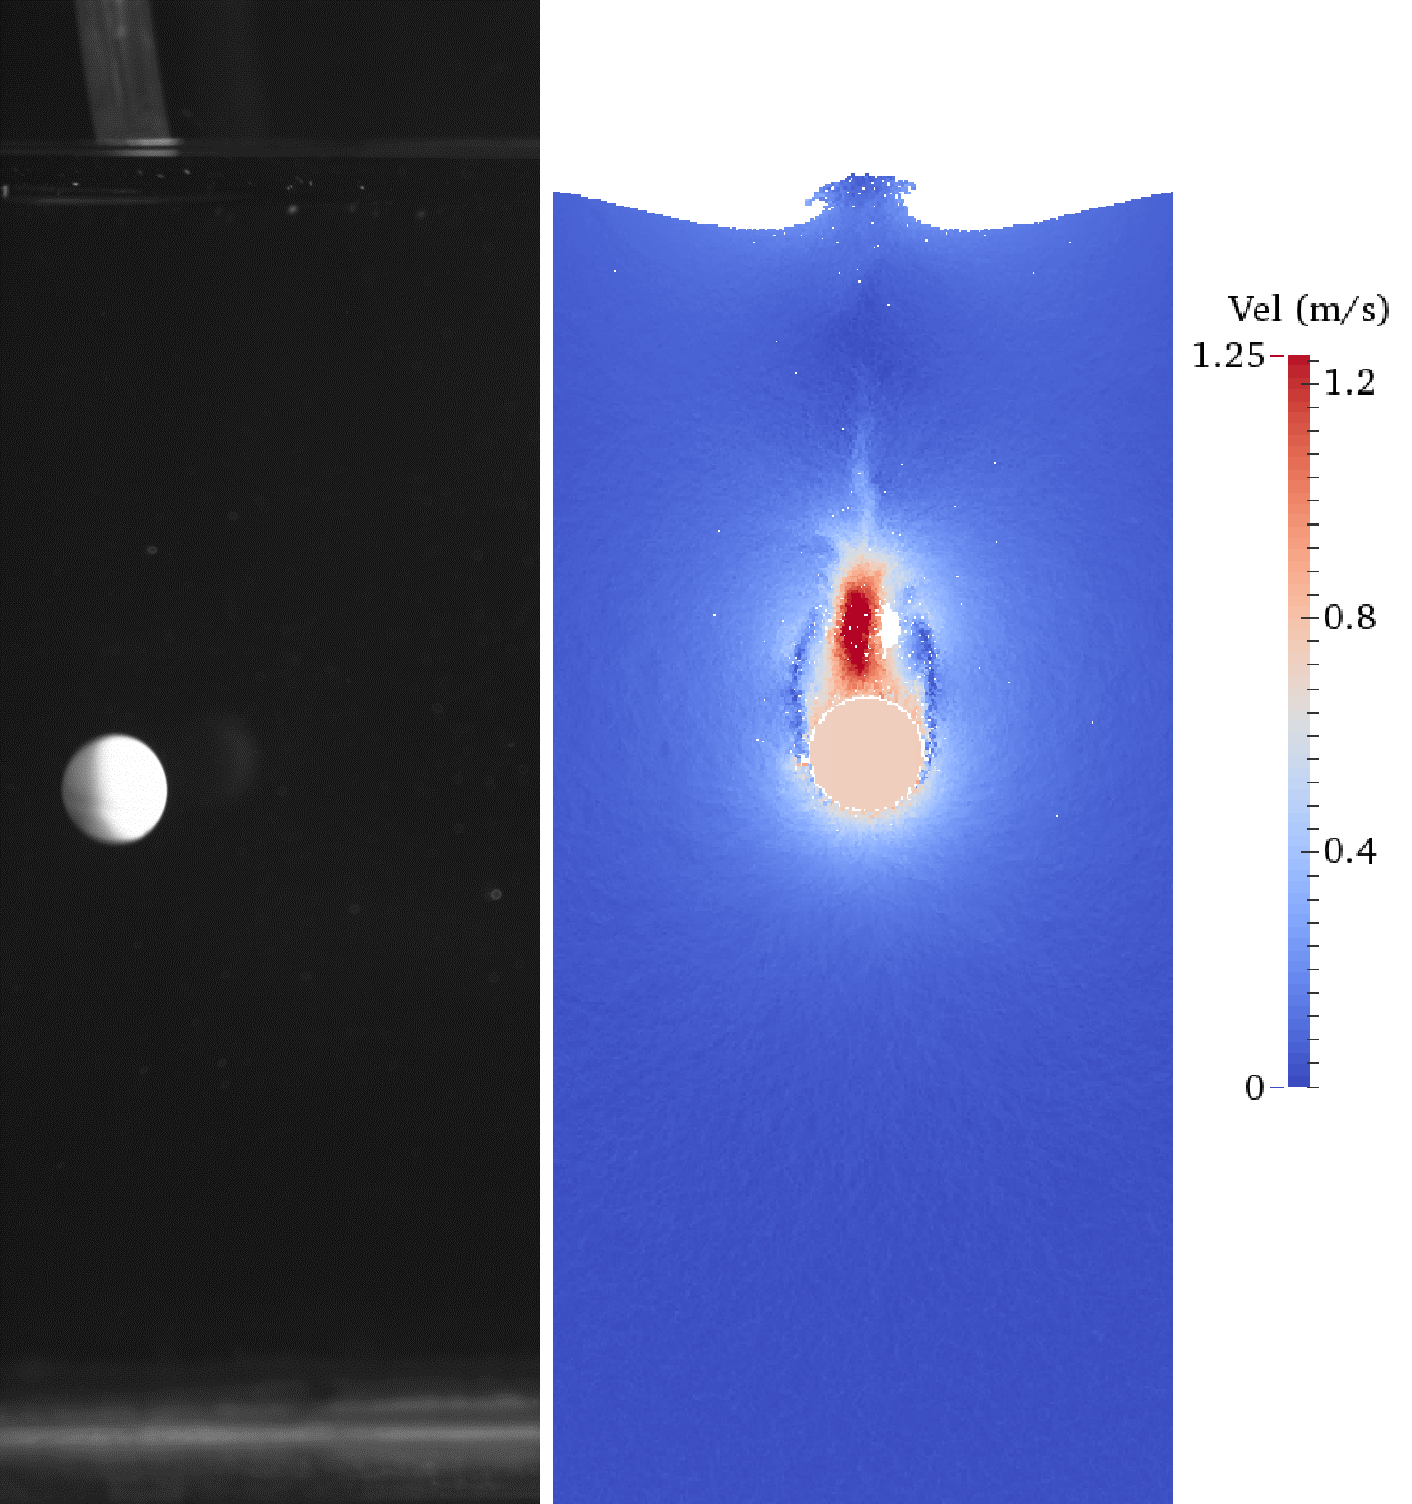
\includegraphics[width=0.48\linewidth]{Figures/5.Chapter/102-8_25_cut}
	\caption{Sinking sphere with $\rho=2.54\rho_{w}$. Experimental and DualSPHysics results. Left $T=6.905$, right $T=8.20$.}
	\label{fig:exp_glass_figs} 
\end{figure}
%
The clearest difference seems to be on the free surface deformation. Although some deformation occurs, the numerical solution greatly over-predicts its magnitude. It is hypothesized that missing surface tension terms in the \ac{SPH} solution are responsible, since at this scale the energy associated with these deformations may be dissipated by these terms. This might be one of the reasons why a slight delay in the sphere movement is visible. As in the cases studied in the previous Section, momentum transfers from the body are required to accommodate the free surface deformation.
Figure \ref{fig:exp_glass} details the evolution of the position and velocities of the sphere.

%
\begin{figure}[ht!]
	\centering
	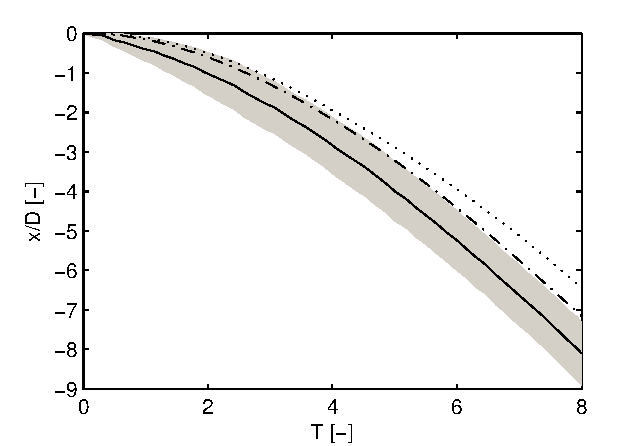
\includegraphics[width=0.48\linewidth]{Figures/5.Chapter/Comp_curve_cut}
	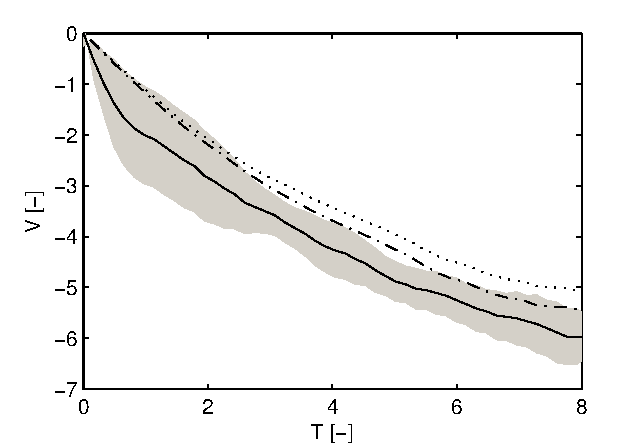
\includegraphics[width=0.48\linewidth]{Figures/5.Chapter/Comp_curve_vel_smooth_cut}
	\caption{Sinking sphere with $\rho=2.54\rho_{w}$. Experimental(-), experimental error region (shaded gray), DualSPHysics $D/Dp=20$ ($\cdots$) $D/Dp=50$ ($- \cdot -$) }
	\label{fig:exp_glass} 
\end{figure}
%

One can see that the more resolved case closely follows the experimental data regarding displacement and shows a good agreement in velocity. 
%After this point there is an inflection in the velocity signal that is not captured by the numerical solutions. {\color{red} Anyone with any idea as to why there is an inflection there? Doesn't seem like bottom influence, still far away, maybe some effect of the turbulent wake? Some eddy detaching?} 
The solution seems to converge and with increasing resolution and with the multi-GPU parallelization better results are expected with higher $D/Dp$ ratios. The periodic conditions at $5D$ distance are also not ideal and may contribute negatively to the solution. Advances on variable resolution schemes with arbitrary 3-D geometries \citep{Vacondio-2013} are also expected to allow for a much more detailed characterization of the flow structures around the object, namely the boundary layer and turbulent wake. For such detailed comparisons with small scale experiments, terms that gain relevance need to be included in the discretization, namely surface tension, as to alleviate the effects in the free surface seen in Figure \ref{fig:exp_glass_figs}.


\subsubsection{Equilibrium position of floating bodies}
\label{subSubsect:equilibrium}

An important scenario is equilibrium position retrieval of floating bodies. It is demanding for a numerical discretization since the system is set in an unstable equilibrium position and is then allowed to evolve until it reaches a stable equilibrium. \cite{Fekken-2004} introduces numerical results for a $0.10\times0.05$ m rectangle, vertically placed in a tank, half submerged, with $\rho=0.5\rho_{w}$. The 2D \ac{SPH} simulations were set with $L/Dp=15$, $L/Dp=30$ and $L/Dp=50$, where $L$ is taken as the smallest side of the rectangle. Figure \ref{fig:349_1_equl} shows the evolution of the system and the angle of the object with the horizontal ($\Theta$) along time, comparing with the data from Fekken. 
%
\begin{figure}[ht!]
	\centering
	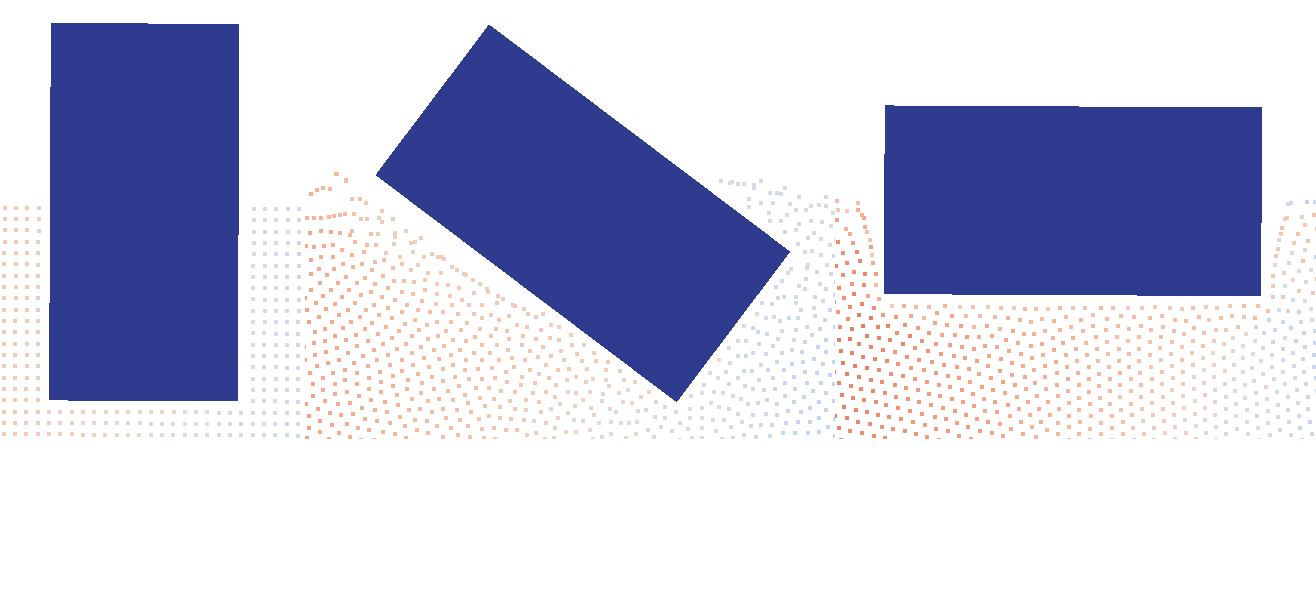
\includegraphics[width=0.50\linewidth]{Figures/5.Chapter/fig19} 
	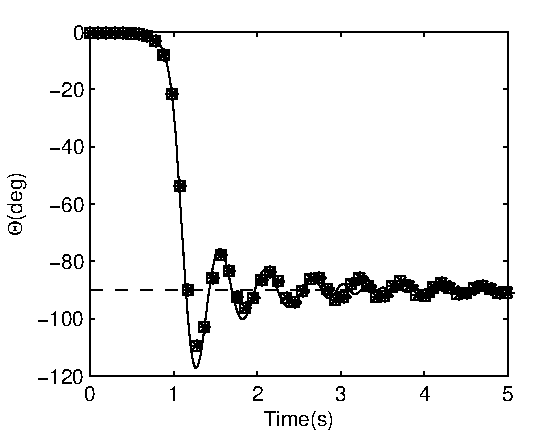
\includegraphics[width=0.49\linewidth]{Figures/5.Chapter/fig20a}
	\caption{Left - Displacement of rectangle at $t=0.0s$, $t=1.1s$ and $t=5.0s$; Right - Angle history of the rectangle. Equilibrium($---$); Fekken(\ac{VOF})\cite{Fekken-2004}($-$); DualSPHysics $L/Dp=15$($\bullet$), $L/Dp=30$($\ast$) and $L/Dp=50$($\Box$).}
	\label{fig:349_1_equl} 
\end{figure}
%

The cylinder correctly finds the stable equilibrium position, at $\Theta=-90$ degrees and the damped oscillatory rotation around that point closely matches the \ac{VOF} results. The more resolved solutions show a marginally better phase matching with the \ac{VOF} results. This result is particularly important since it shows that the system avoids unstable positions, correctly reproduces the dynamics of the event and is robust even with low resolution simulations. Unlike on the \ac{VOF} simulations, no acceleration was imposed in the first instants of the simulation in order to force the system to diverge from the initial position: the \ac{SPH} solution instabilizes by itself. This appears to be a result of the large amount of interactions involved in every time-step and the initial cubic lattice used for particle positioning. Small errors owing to machine precision and non-repeatability of the thread order of the parallel implementation \citep{Dominguez-2013a} causes very small numerical unbalances, that would otherwise be diffused, to be amplified by the physically unstable configuration of the system.


%%%%%%%%%%%%%%%%%%%%%%%%%%%%%%%%%%%%%%%%%%%%%%%%%%%%%%%%%%%%%%%%%
\subsection{Normal Dry Collisions}
\label{sec:validation_dry_collision}

The results compiled by \cite{Kruggel-Emden-2007} show the dependency of the restitution coefficient with velocity to be in line with $(1-e_n)\sim v_{n}^{1/5}$. The used non-linear Hertzian model described by Equations \eqref{eq:non_linear_hertz_normal} to \eqref{eq:gamma_dem} was derived in the prospect of complying with experimental data. Qualitatively, Figure \ref{fig:e_hertz} shows a dependency with the correct tendencies, but the model parameters may influence the accuracy of the force computation, depending on the materials in question. Furthermore, forces are used to update the dynamics of the rigid bodies with Equations \eqref{eq:rigid_linear} and \eqref{eq:rigid_angular}, that are then integrated in time.

Data was collected using 3D simulations, where a sphere, with diameter $D$, hits a wall made of the same material, in the normal direction, with a given launch velocity $V_0$. Zero body forces imply that the only forces acting on the dynamics of the system are the normal contact forces, correctly replicating the pendulum conditions of the experimental work. Three materials are tested: steel, aluminum and lead. Table \ref{tab:material_props} condenses the parameters used in the simulations.
%
\begin{table}[h]
\centering
\begin{tabular}{l|lll}
 & $E\;[Nm^{-2}]$ & $\nu_p\;[-]$  & $e\;[-]$ \\ \hline
Steel & $200\times10^9$ & $0.30$ & $0.85$ \\
Aluminum & $65\times10^9$ & $0.33$ & $0.75$ \\
Lead & $16\times10^9$ & $0.42$ & $0.40$
\end{tabular}
\caption{Young modulus, Poisson coefficient and restitution coefficient used in the simulations.}
\label{tab:material_props}
\end{table}
%

Of special notice should be the restitution coefficient, $e$, used to define the viscous damper coefficient in Equation \eqref{eq:gamma_dem}. It should be understood, in the context of our non-linear model, as a tuning parameter, with a purely numerical meaning. By varying the initial velocity $V_0$ and measuring the velocity after the impact, $e_n$ was measured, as given by Equation \eqref{eq:rest_coeff_def}, resulting in Figure \ref{fig:Restitution_coeff_dem}.

%
\begin{figure}[ht!]
	\centering
	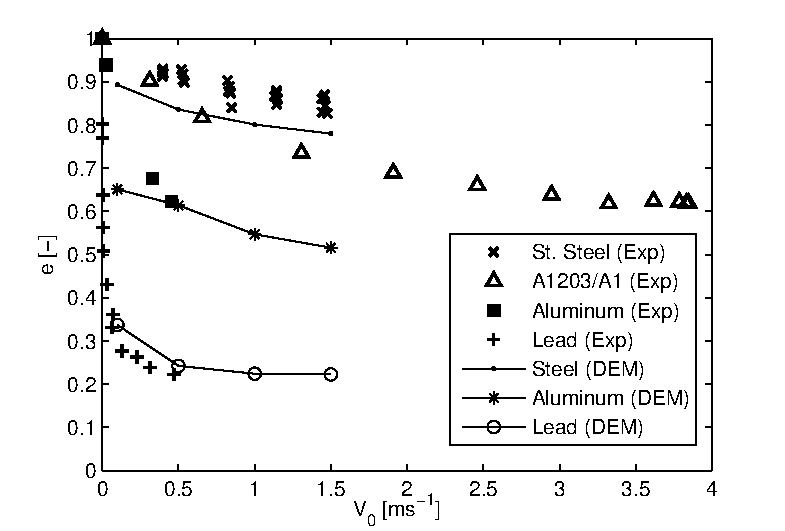
\includegraphics[width=0.70\linewidth]{Figures/5.Chapter/e_vo_DEM}
	\caption{Restitution coefficient $e$ as a function of initial normal velocity $V_0$. Experimental data \citep{Kruggel-Emden-2007} and numerical solution.}
	\label{fig:Restitution_coeff_dem} 
\end{figure}
%

There seems to be good agreement in the range of values obtained, as well as the tendency inverse relation between $e_n$ and the impact velocity. The results are independent from resolution, and were tested with $D/Dp=10$, $D/Dp=50$ and $D/Dp=150$, with variations of less than $1\%$ in $e_n$. As $V_0$ tends to zero, the numerical $e_n$ does not converge so rapidly to 1 as in the experimental data. Both shortcomings in the adopted model and the difficulty of accurately measuring very small velocities in an experimental context lead to a difficult debate on the origin of the differences.


%%%%%%%%%%%%%%%%%%%%%%%%%%%%%%%%%%%%%%%%%%%%%%%%%%%%%%%%%%%%%%%%%
\subsection{Experimental Validation: Dam-break with moving obstacles}
\label{sec:validation_exp}

The Wave Channel of the Hydraulics laboratory (LHIST) of the Civil Engineering Department at Instituto Superior T\'{e}cnico, Lisbon, Portugal, was adapted to perform dam break tests. The flume was sectioned at 8.0 m long and is 0.70 m wide, with glass side walls in order to grant optical access to the flow. The flume material can be considered very smooth both in the walls and the bed. A gate was installed, as seen in Figure \ref{fig:Gate_channel}.
%
\begin{figure}[ht!]
	\centering
	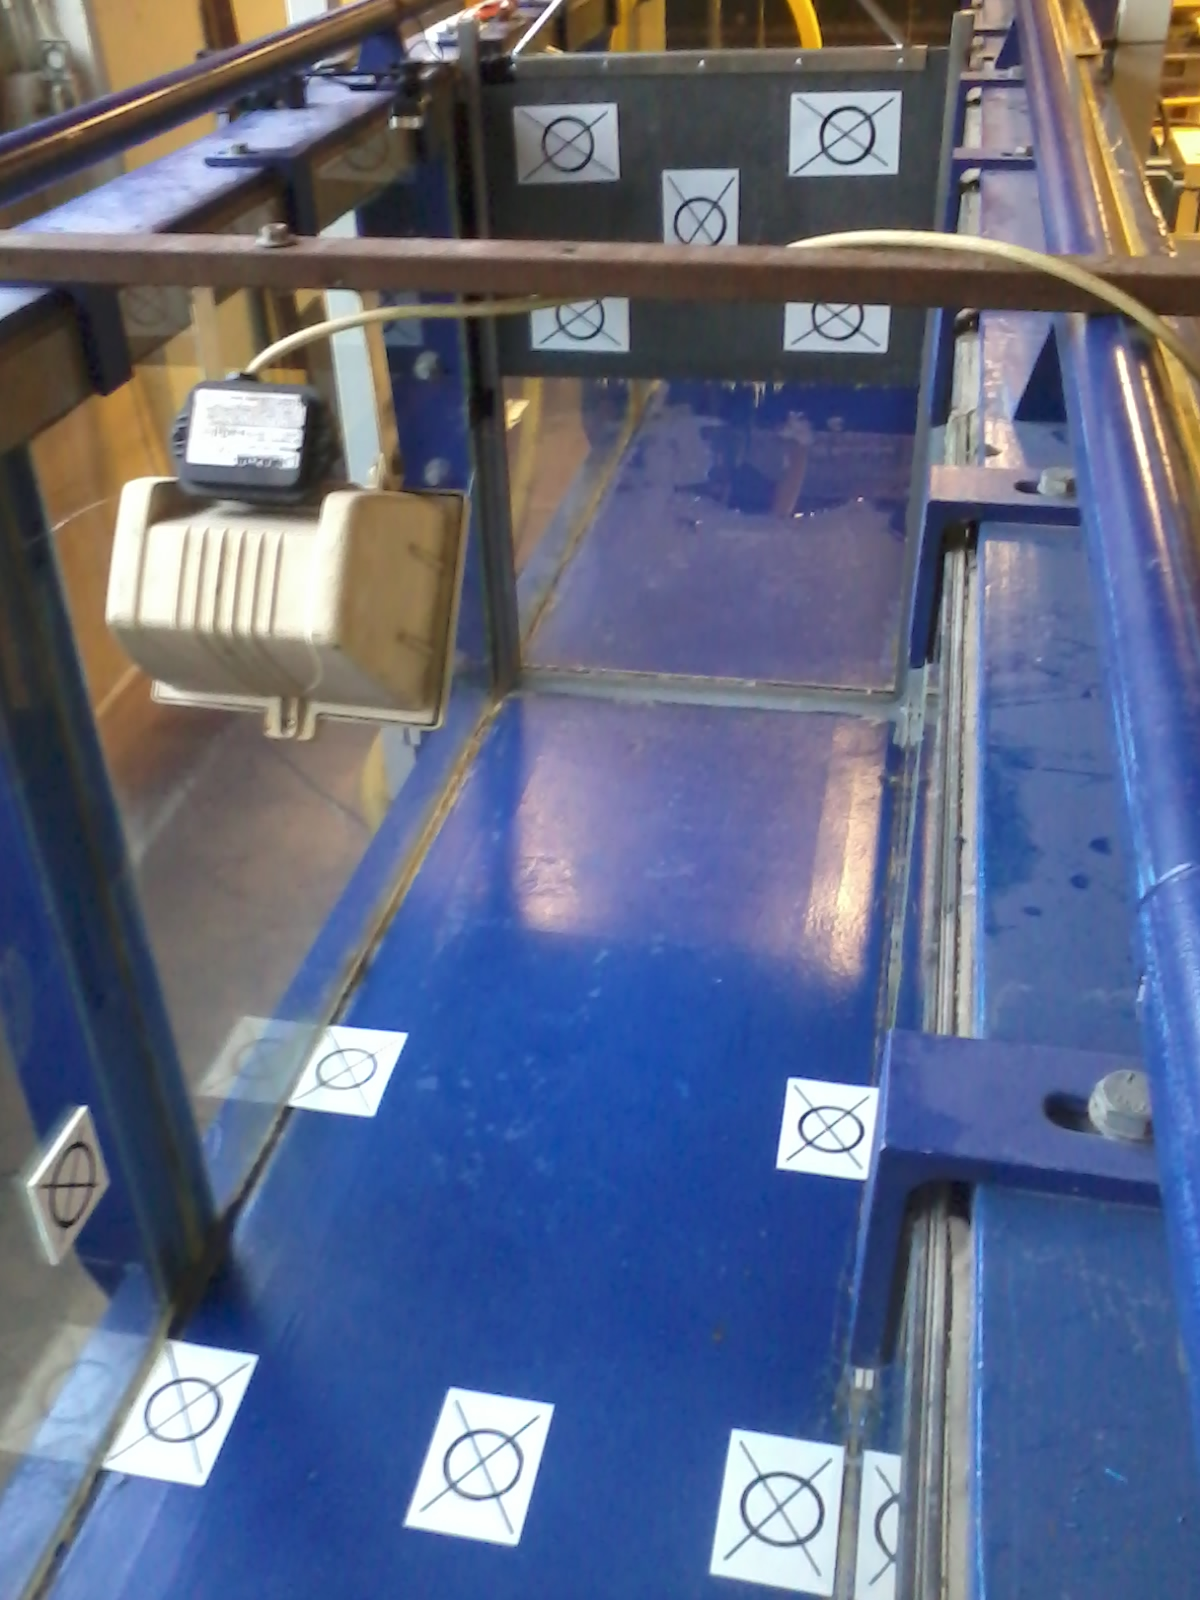
\includegraphics[width=0.45\linewidth]{Figures/5.Chapter/Gate_channel} 
	\caption{Upstream perspective of the channel and the open gate.}
	\label{fig:Gate_channel} 
\end{figure}
%

Together with a lock lever and a monolithic weight, the pulley system allowed for opening action that was easily repeated and provided an 'instantaneous' removal for the dam-break. The measured opening time was $0.21$ s, lesser than the required theoretical limit for a dam break $t_o(h_0=0.40)=\sqrt{2h_0/g}\approx0.29$ s \citep{Lauber-1998}.

A series of PVC cubes with a $L=0.15$ m side, filled with a material that resulted in a final density of $800\;\text{kgm}^{-3}$, were built. These were sealed to ensure that the content of the cubes remained dry, with regular mass measures performed during the experiments.

Three synchronized video cameras pointing from the upstream, top and downstream directions provide means to track the cubes as the flow progresses. A \ac{DTL} implementation \citep{Capel-matlab-dlt} was adapted, providing inverse homography and error quantities. Since only two images are needed to estimate the objects coordinates and three are provided, the error measure is taken as the deviation from the results from the tree possible pairs. Targets are observable in Figure \ref{fig:Gate_channel}. These are placed on flume bed and walls at known positions, providing means for camera calibration and reference points for the reconstruction algorithm. A flash triggered with the release of the gate marked the synchronization time for the several cameras.

Several configurations of the stacked cubes were tested, as indicated in Figure \ref{fig:lab_configs}.
%
\begin{figure}[ht!]
	\centering
	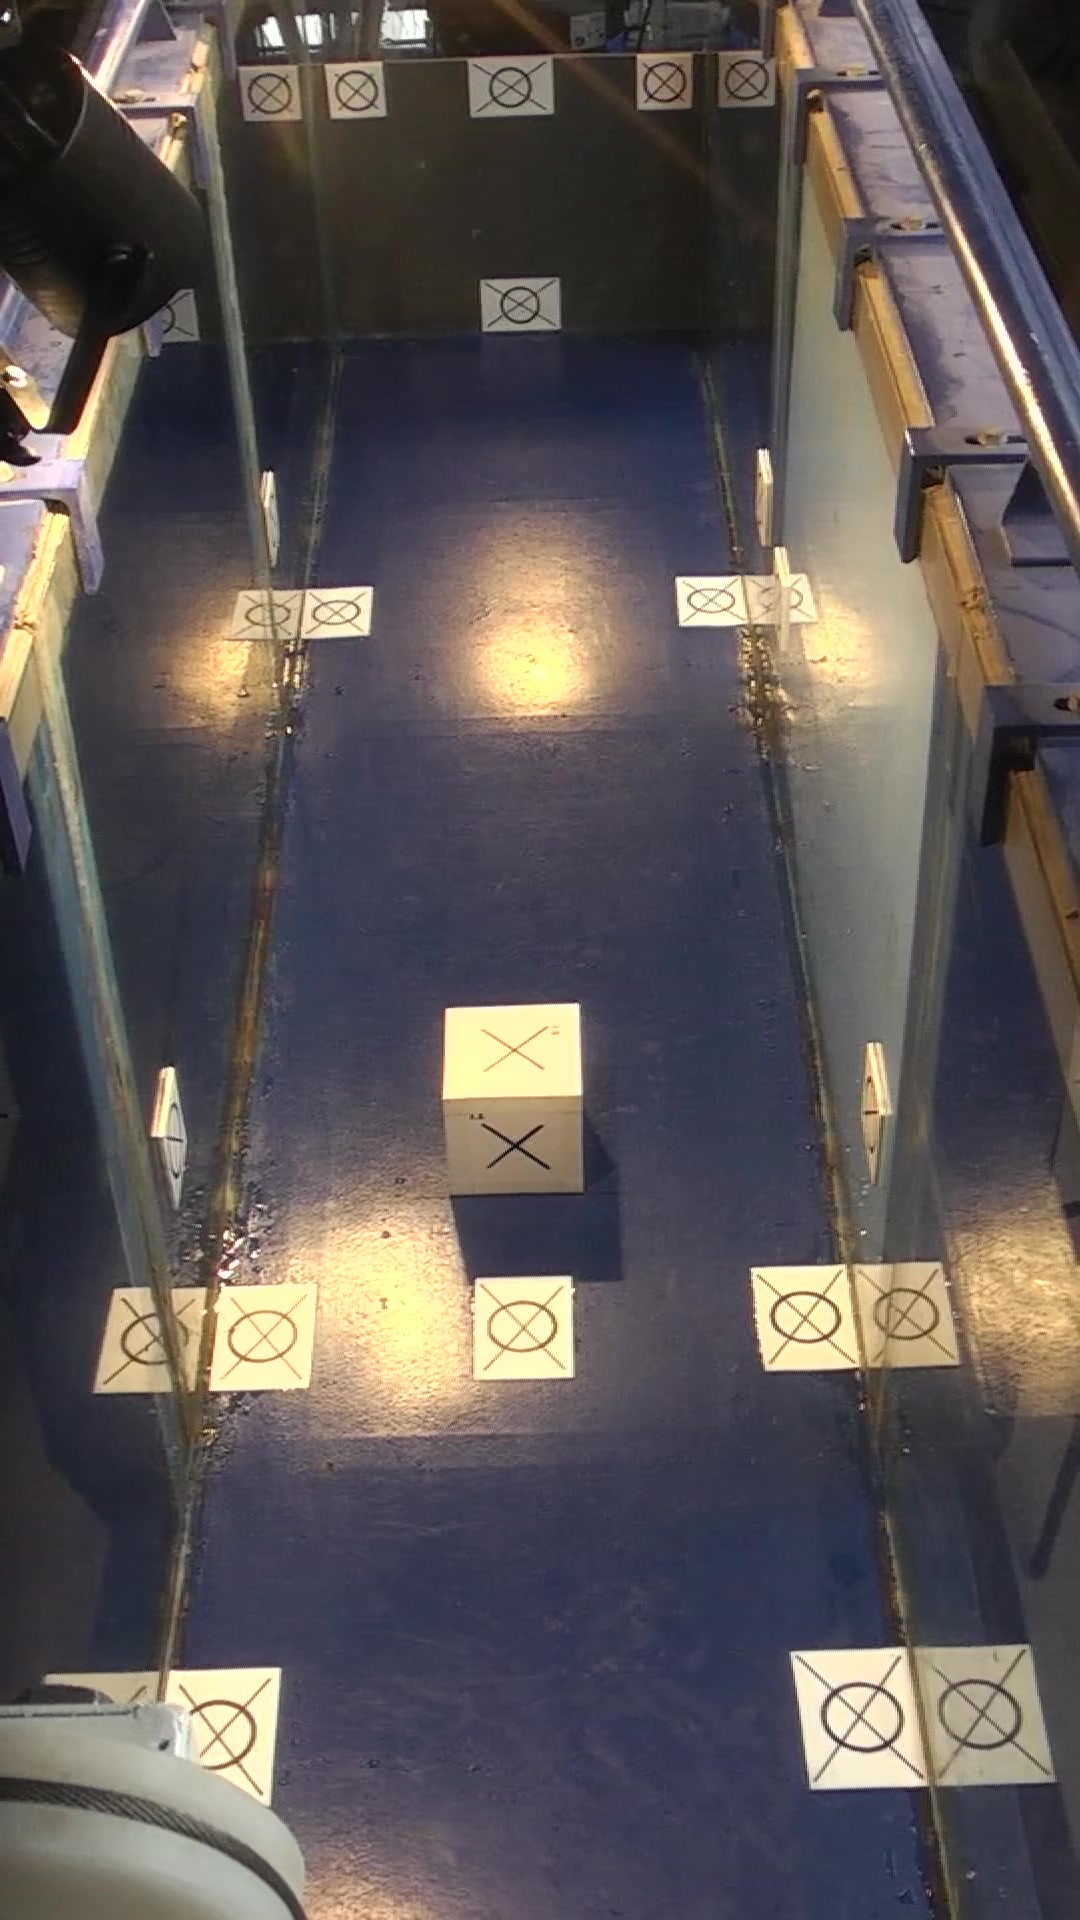
\includegraphics[width=0.28\linewidth]{Figures/5.Chapter/fig_2a} 
	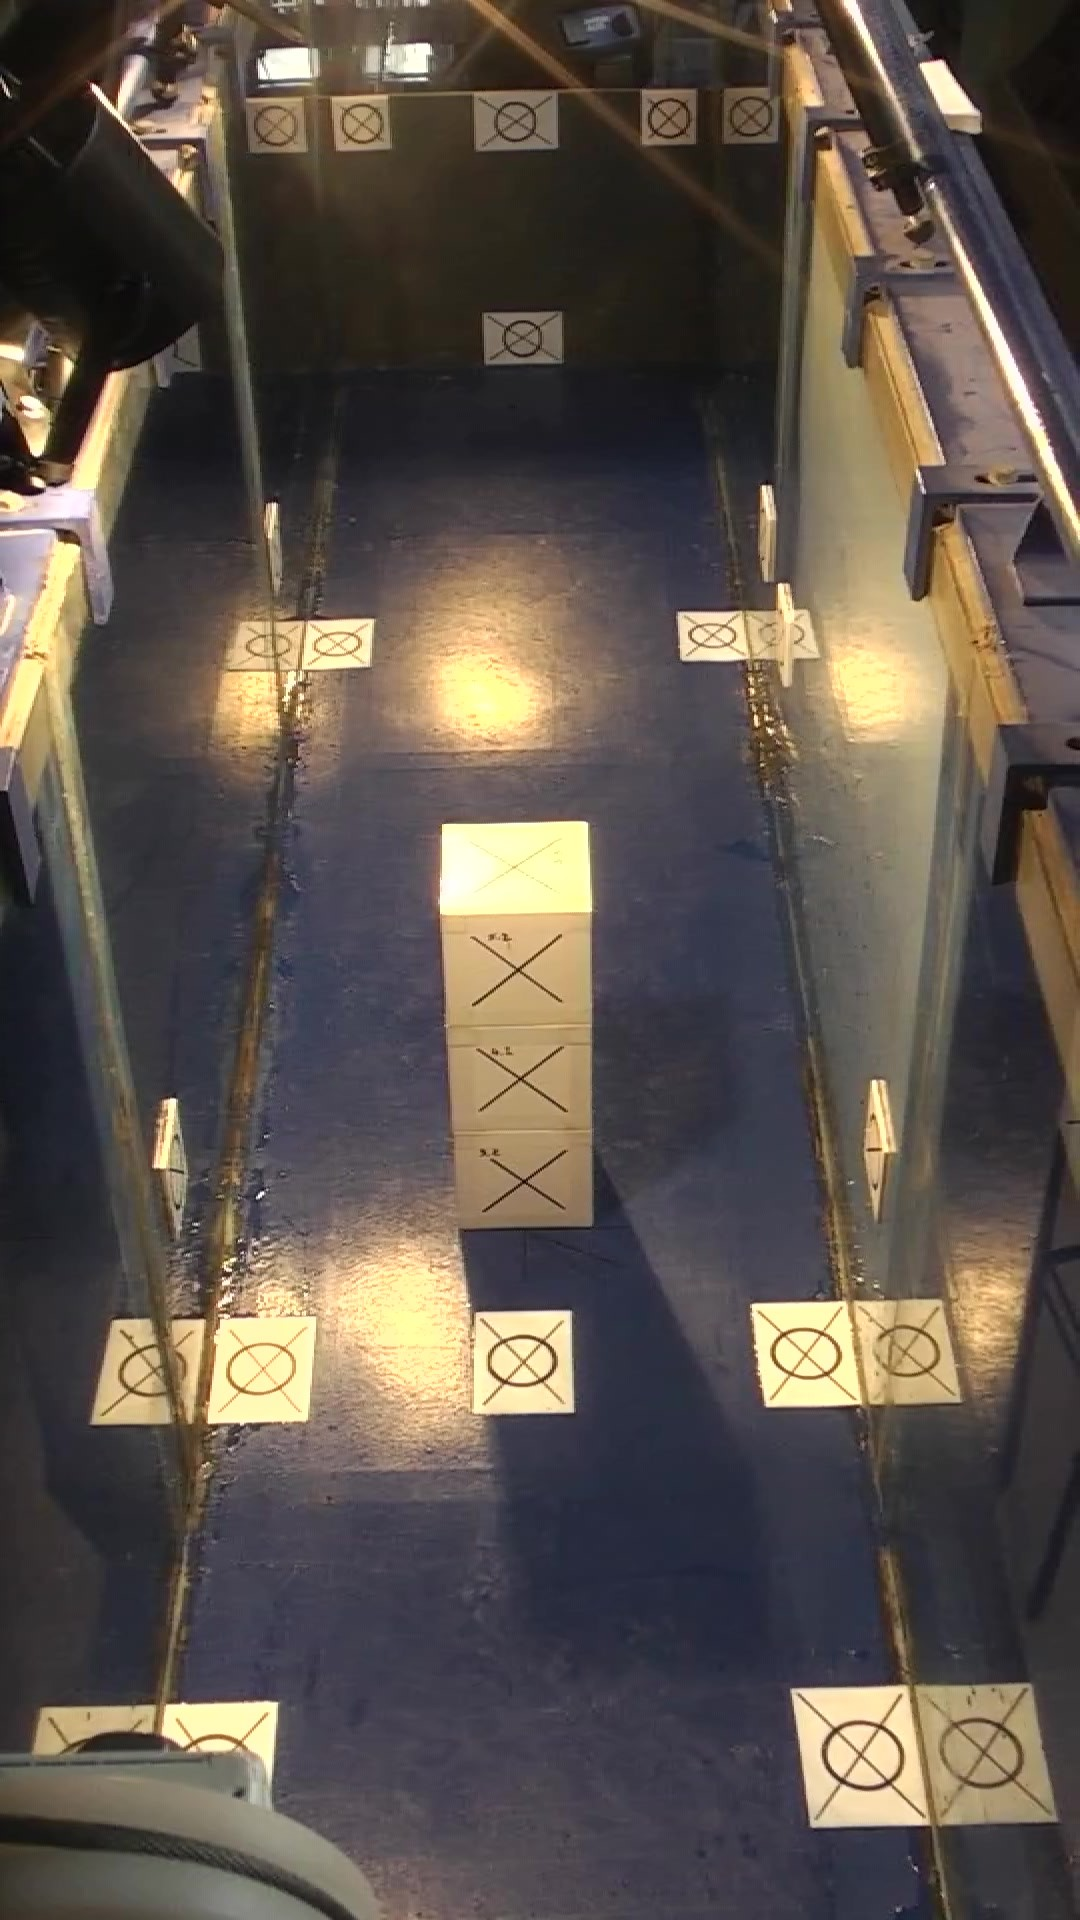
\includegraphics[width=0.28\linewidth]{Figures/5.Chapter/fig_2b}
	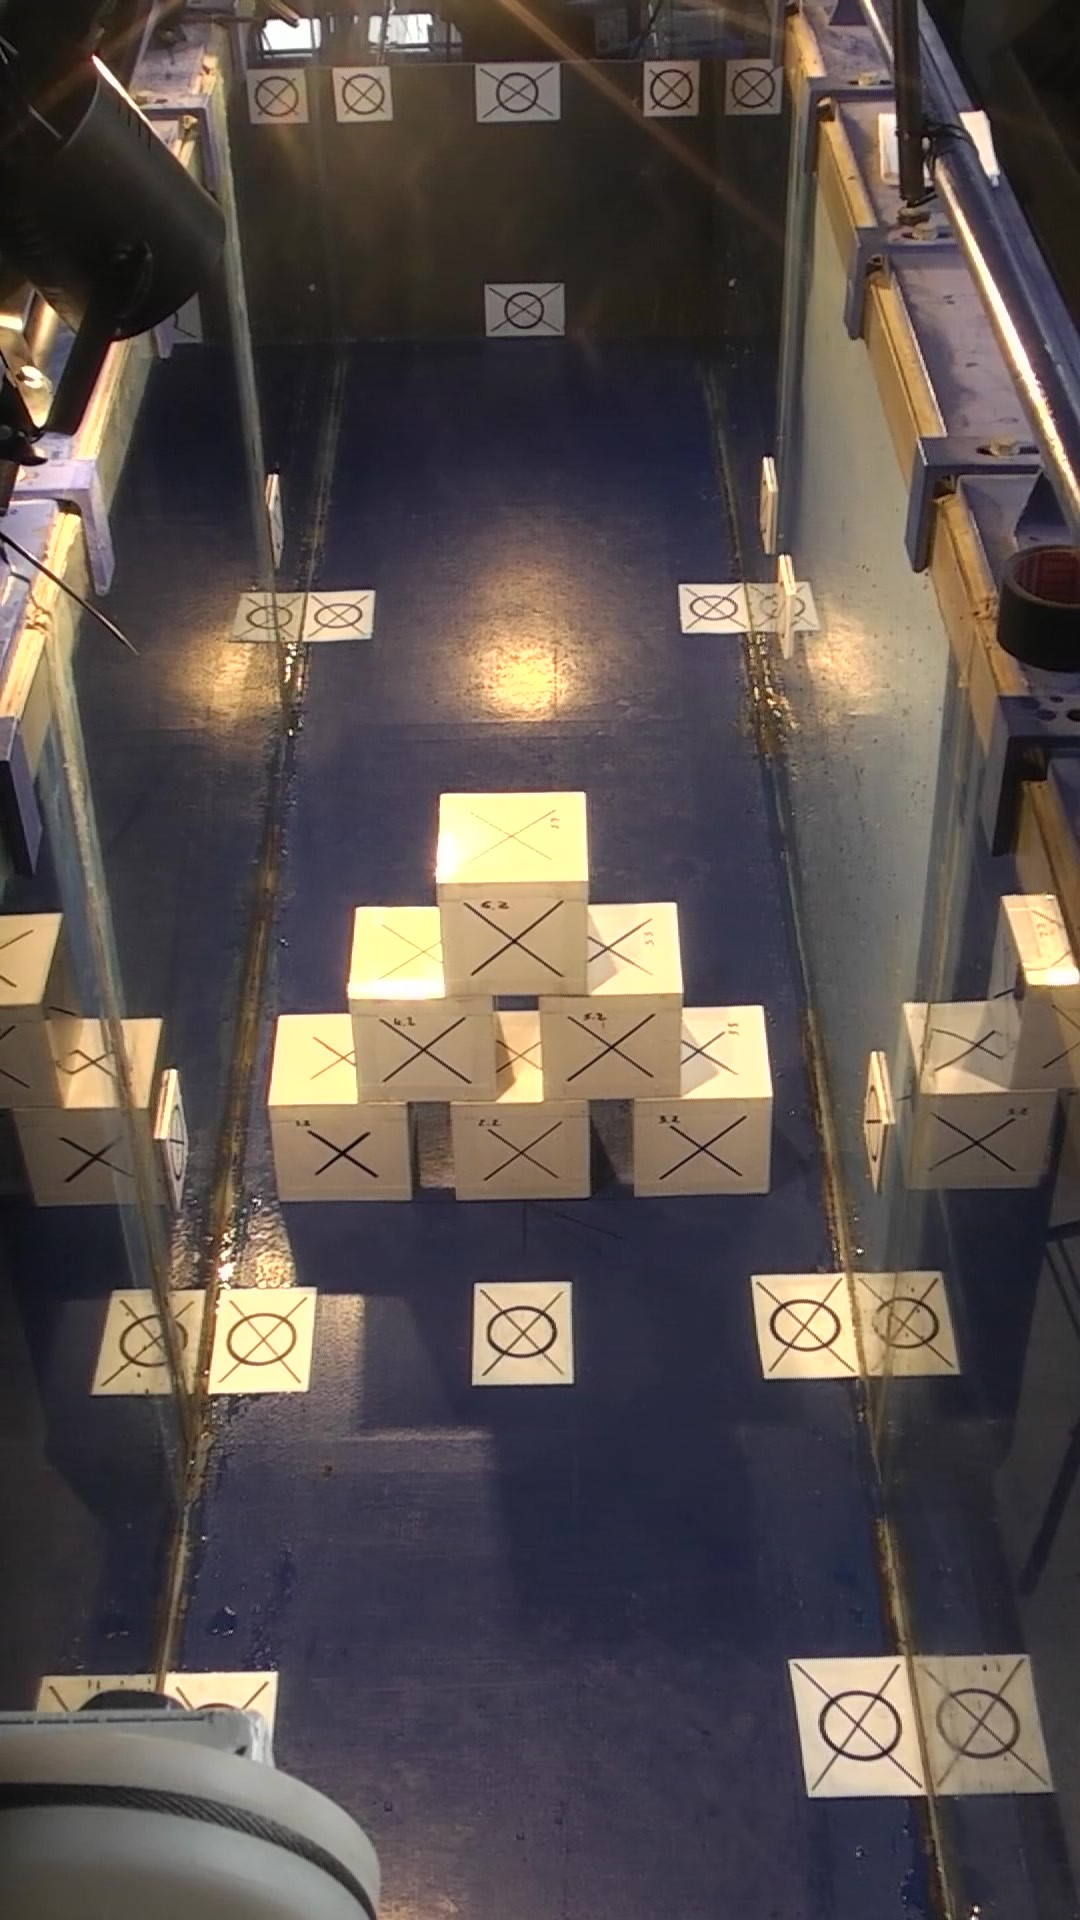
\includegraphics[width=0.28\linewidth]{Figures/5.Chapter/fig_2c}
	\caption{Three cube configurations, Left - I, Center - II, Right - III}
	\label{fig:lab_configs} 
\end{figure}
%

The origin of the reference system was chosen as the right bottom at the gate section. The $x$ axis extends along the flume in the downstream direction, $z$ axis points upward and the $y$ axis points right.

Each configuration was measured twice in order to establish a measure of the repeatability of the experiments. With both measurements and considering that each run can be tracked with three pairs of images six virtual runs by configuration can be measured.

Using configuration I, \ac{PIV} measurements were performed on the locus of the impact of the wave with the objects, allowing for a visualization of the velocity field, presented in Section \ref{Subsect:PIV}.

\subsubsection{Configuration I}
\label{Subsect:config_I}
%
Case I presents a single cube in the center of the flume, with a face directly aligned with the flow direction. The numerical solution must be able to generate a correct equilibrium position for the cube, balancing the gravity force by producing a contact force. Initial conditions do not include contact forces, as they are computed at the expense of small displacements (DEM with soft-body approach) of the particles that make up the rigid body. 

Parameters in Equations \eqref{eq:non_linear_hertz_normal} to \eqref{eq:fric_I} were set to represent the various materials in the simulation, as described in Table \ref{tab:material_props_cubes}.
%
\begin{table}[h]
\centering
\begin{tabular}{l|l|llll}
 & Material & $E\;[Nm^{-2}]$ & $\nu_p\;[-]$  & $e\;[-]$ & $\mu_f\;[-]$\\ \hline
Flume bottom & Steel & $200\times10^9$ & $0.30$ & $0.85$ & $0.35$ \\
Walls & Glass & $65\times10^9$ & $0.23$ & $0.80$ & $0.40$ \\
Cubes & PVC & $3\times10^9$ & $0.30$ & $0.40$ & $0.45$
\end{tabular}
\caption{Young modulus, Poisson coefficient, restitution coefficient and friction coefficient used in the simulations.}
\label{tab:material_props_cubes}
\end{table}
%

For all simulations the smoothing length was $h=1.2\sqrt{3Dp^2}$, the $C$ parameter from the stability region condition, Equation (\eqref{eq:sph_stability_region}), was set at $0.20$ for all simulations and the kinematic viscosity is that of water at $20^{\circ}$ C temperature, $\nu = 10^{-6} \  \mathrm{m^2 s^{-1}}$.

The cube positions along the longitudinal dimension from the numerical solution are plotted against the experimental measures in Figure \ref{fig:cube1_d2_I}.
%
\begin{figure}[ht!]
	\centering
	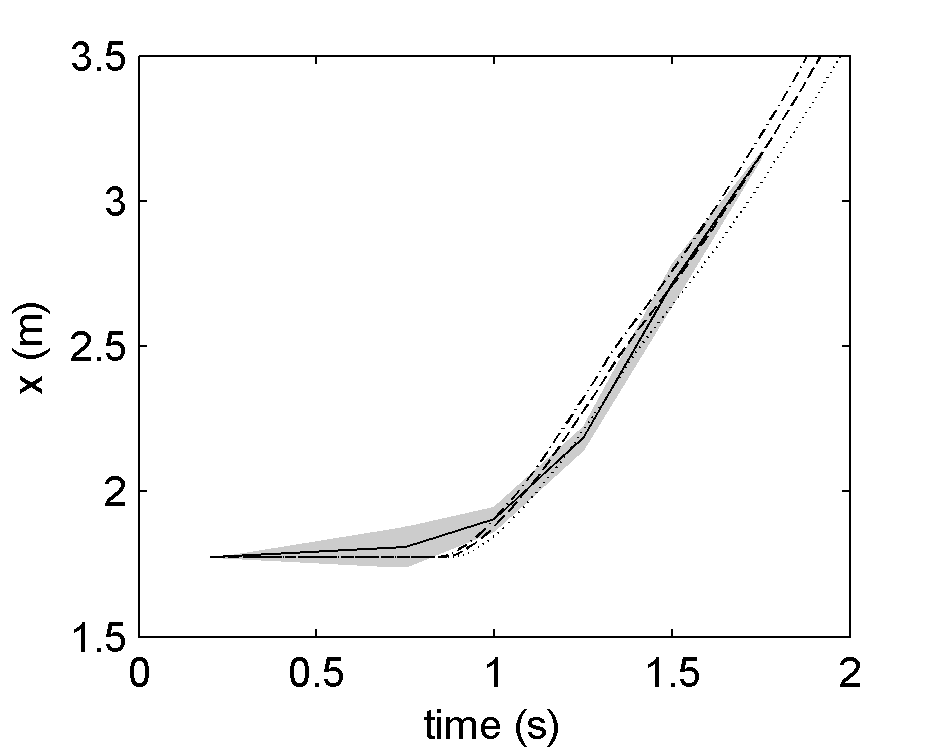
\includegraphics[width=0.45\linewidth]{Figures/5.Chapter/Fig_3}
	\caption{$x$ coordinates in time. Experimental (-), DualSPHysics $L/Dp=10 (- \cdot -)$, $L/Dp=15 (- -)$, $L/Dp=45 (\cdots)$.}
	\label{fig:cube1_d2_I} 
\end{figure}
%

The shadowed area represents the symmetrical error region obtained by considering the variation obtained between the two consecutive experimental runs, plus the variation between measurements in the same run. The comparison shows good agreement between experimental and numerical data, implying that both normal and frictional forces are accurately computed. The frictional mechanism seems to correctly predict the transition from static to dynamic situations, showing that the Coulomb limit is applicable. Increasing the resolution from $L/Dp=10$ to $L/Dp=45$ renders small variations on the results, maintaining the positive agreement with the experimental data.


\subsubsection{Configuration II}
\label{Subsect:config_II}
%
Configuration II presented three stacked cubes directly aligned with the flow direction. This configuration attests to the capability of the model to respect static equilibrium positions of stacked objects. No kinematic restrictions are applied, forces are computed dynamically but their resultant is equal to the gravity force and other forces applied. Again, initial position adjustments are minimal since the springs in Equation \eqref{eq:non_linear_hertz_normal} are very rigid. No vibrations due to over-shoot and under-shoot cycles are detected due to the effectiveness of the viscous damping term. Figure \ref{fig:figs_D2_III} shows a frame from the experiment aligned with the numerical solution in the same instants. Note that for visualization convenience an isosurface derived from the SPH solution is plotted.
%
\begin{figure}[ht!]
	\centering
	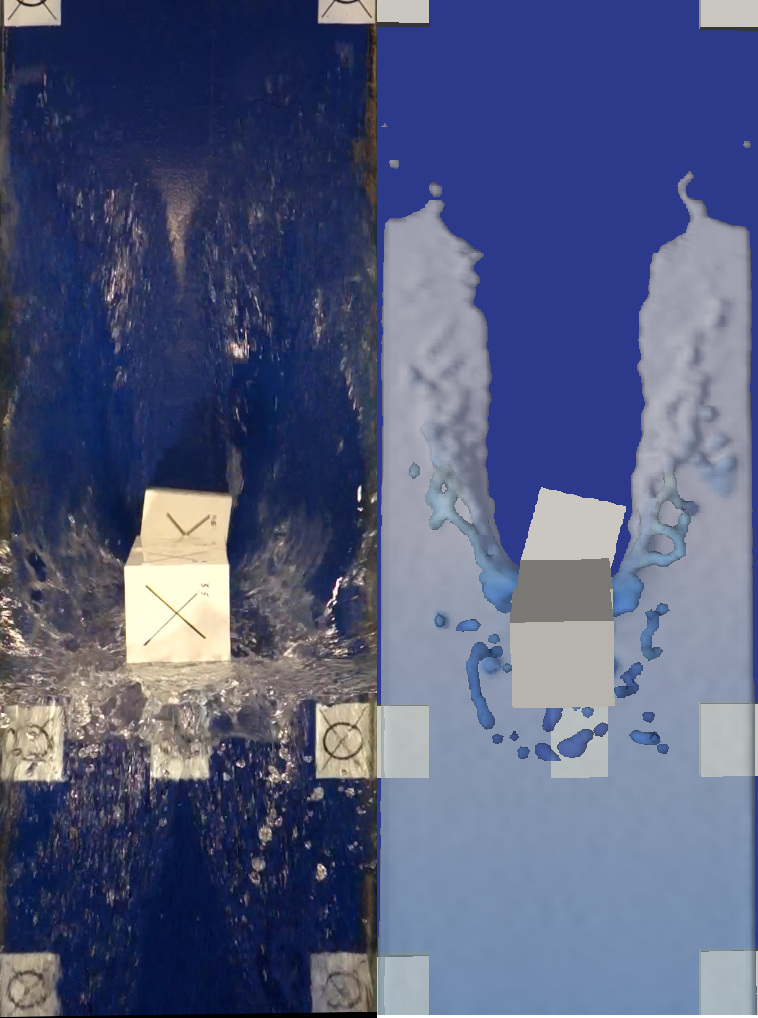
\includegraphics[width=0.35\linewidth]{Figures/5.Chapter/Fig_4a}
	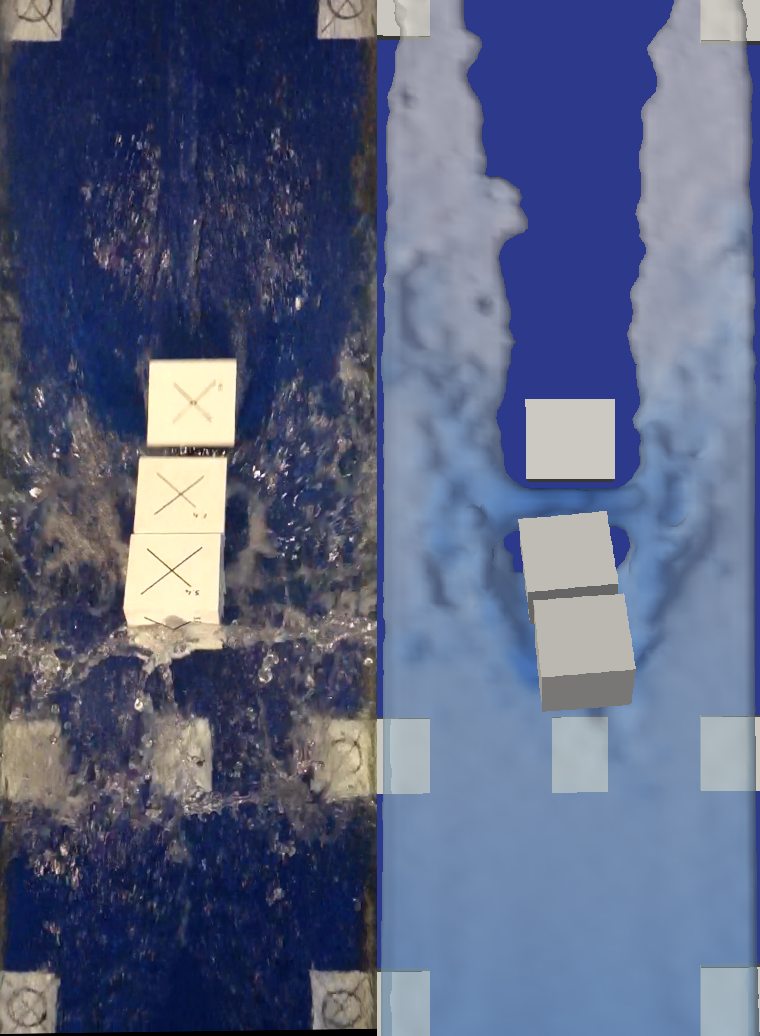
\includegraphics[width=0.35\linewidth]{Figures/5.Chapter/Fig_4b}
	\caption{Configuration II. Experimental $vs$ numerical rendering of solution. Left $t=0.98s$, right $t=1.28s$.}
	\label{fig:figs_D2_III} 
\end{figure}
%

The bottom cube presents as main direction of movement the longitudinal axis, much as the cube of Configuration I, but here more complex phenomena are present. The involved forces must now also account for the weight of the top cubes, multiplying the order of magnitude of the frictional components in the beginning of the movement. Figure \ref{fig:cube1} shows the evolution of the cube coordinates, where once again the shadowed area represents the experimental variability.
%
\begin{figure}[ht!]
	\centering
	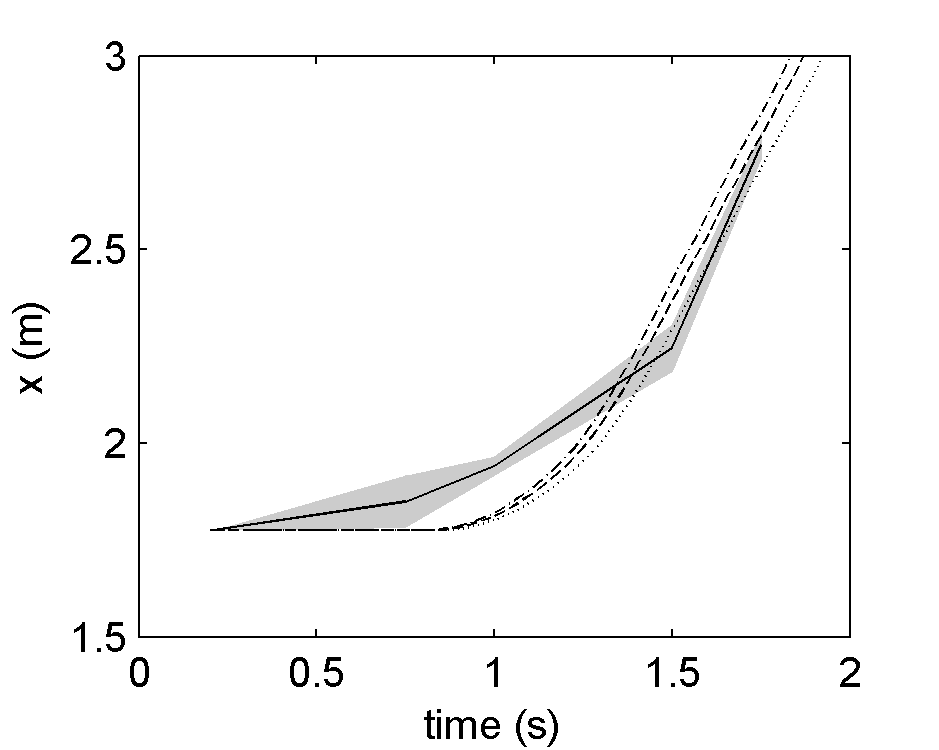
\includegraphics[width=0.45\linewidth]{Figures/5.Chapter/Fig_5}
	\caption{Bottom cube. $x$ coordinates in time. Experimental (-), DualSPHysics $L/Dp=10 (- \cdot -)$, $L/Dp=15 (- -)$, $L/Dp=45 (\cdots)$.}
	\label{fig:cube1} 
\end{figure}
%

The agreement is positive, while the initial instants of motion are not fully recovered. Frictional force on the bottom and upper faces seems to be over predicted, resulting in a delay of around $0.5s$ before static friction, given by the spring-damper mechanism (Equation \eqref{eq:elastic_fric}), is limited by the Coulomb force (Equation \eqref{eq:fric_I}). Once in motion, as in Configuration I, the velocity is in good agreement with the measurements, again indicating that kinematic friction is well accounted for. Increasing resolution does not improve the behavior of the initial instants. The top cube provides two characteristic motion directions, along the $x$ and $z$ axis, as the cube falls after the stack looses integrity. Figure \ref{fig:cube3} quantifies the motion along these axis.
%
\begin{figure}[ht!]
	\centering 
	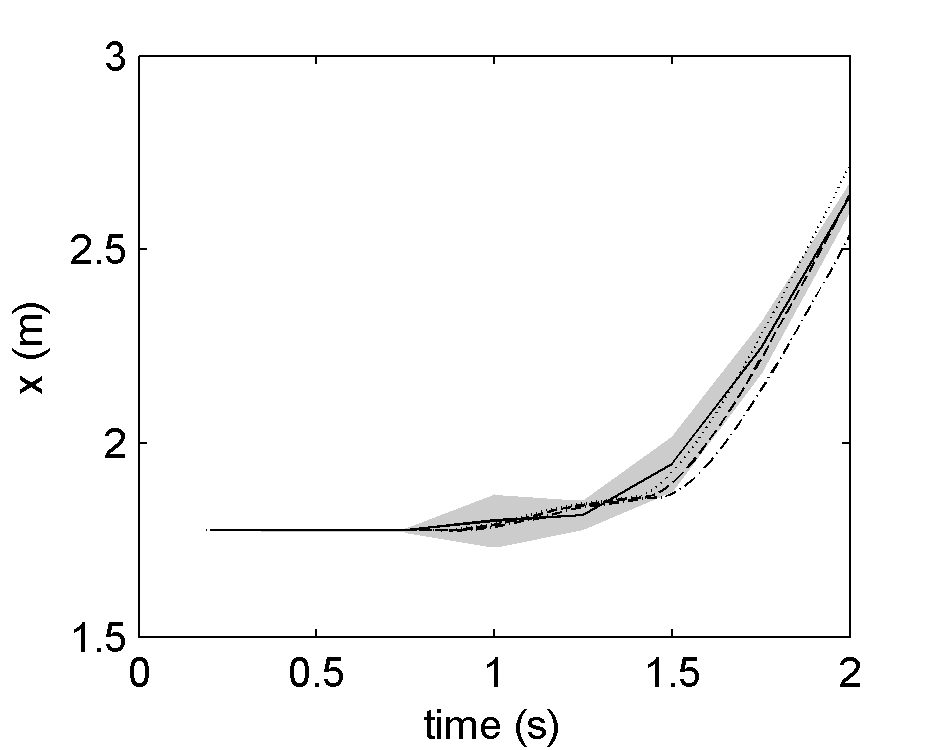
\includegraphics[width=0.45\linewidth]{Figures/5.Chapter/Fig_6a}
	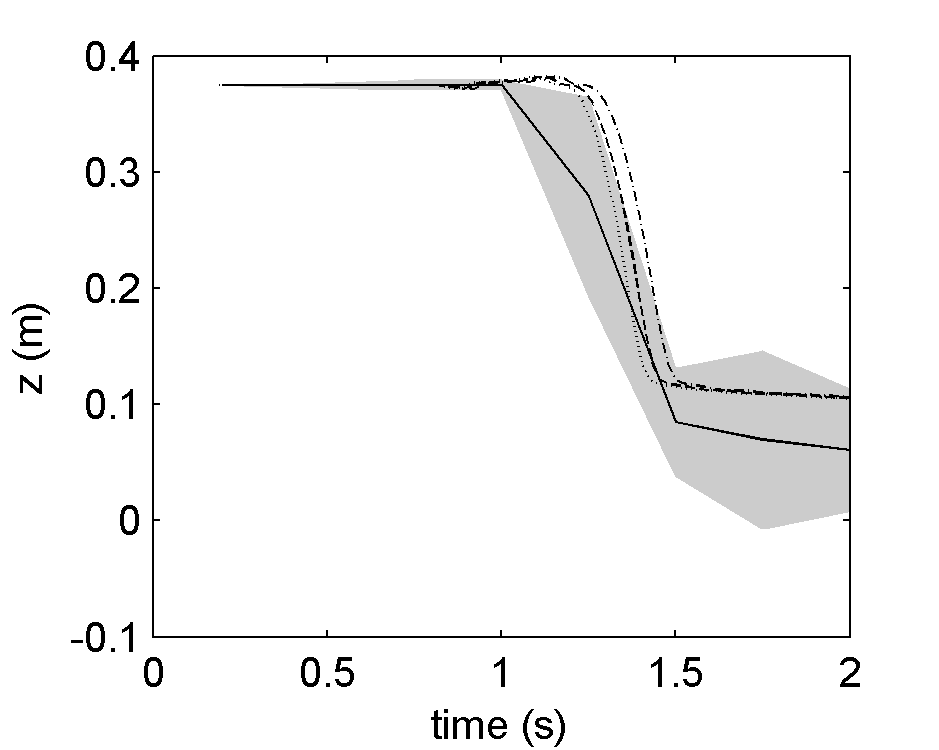
\includegraphics[width=0.45\linewidth]{Figures/5.Chapter/Fig_6b}
	\caption{Top cube. Left - $x$ coordinates, Right - $z$ coordinates. Experimental (-), DualSPHysics $L/Dp=10 (- \cdot -)$, $L/Dp=15 (- -)$, $L/Dp=45 (\cdots)$.}
	\label{fig:cube3} 
\end{figure}
%

Motion along the $x$ axis is very well predicted, with initiation of motion, initial velocity given by the momentum imprinted by friction from the middle cube and velocity once dragging starts being well represented. A small delay in the initiation of the dragging is noticed, but a correct velocity seems to be recovered. The increased resolution seems to effectively correct the delay and further improve the final velocity. Along the $z$ axis, the bulk of the motion is well predicted, but the initiation of the fall is delayed due to a vertical component of momentum being transferred to the cube, effectively sustaining it at the initial position for longer. Such behavior seems to be the result of high frequency oscillations in the force chain of the rigid cubes, leading to an accumulation of energy that the contact dampers are not able to dissipate. Similar phenomena were reported by \cite{Cummins-2011}, that concluded that it is a direct consequence of considering rigid bodies with no internal dissipation mechanisms.


\subsubsection{Configuration III}
\label{Subsect:config_III}

Configuration III represents a highly complex geometry, with a pyramid of cubes forming a wide obstacle on the flume. Gaps between the cubes further complicate the case, by allowing fluid to exert forces not only frontally but also laterally, between cubes. Figure \ref{fig:figs_D2_IV} shows two frames from the experimental runs and the equivalent numerical solutions.
%
\begin{figure}[ht!]
	\centering 
	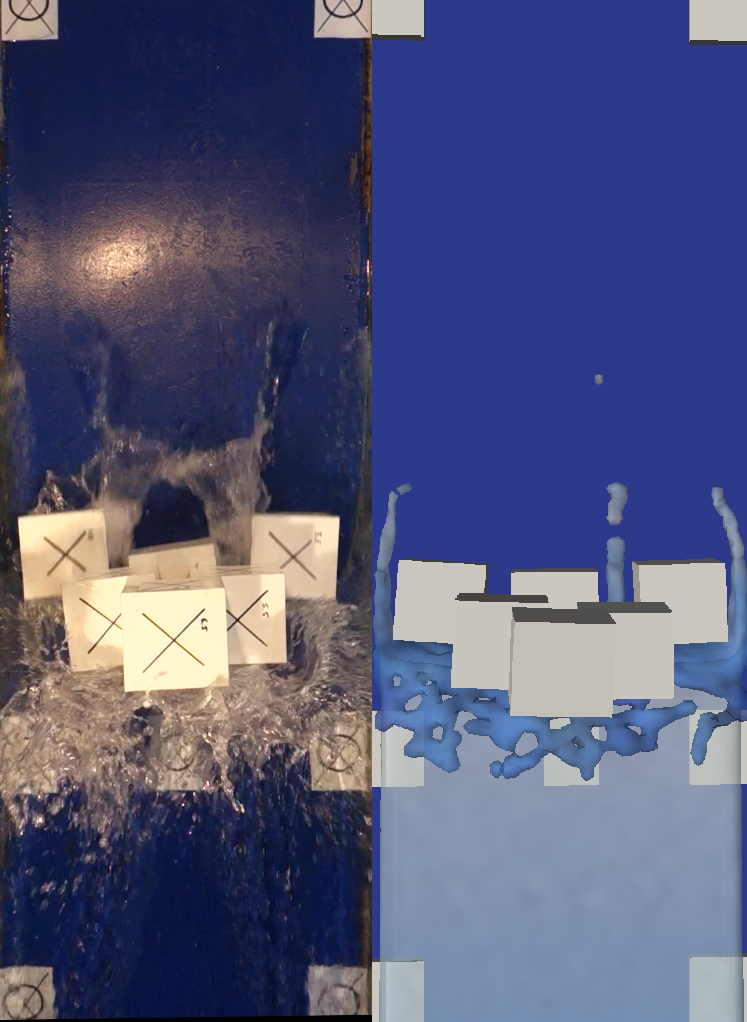
\includegraphics[width=0.35\linewidth]{Figures/5.Chapter/Fig_7a}
	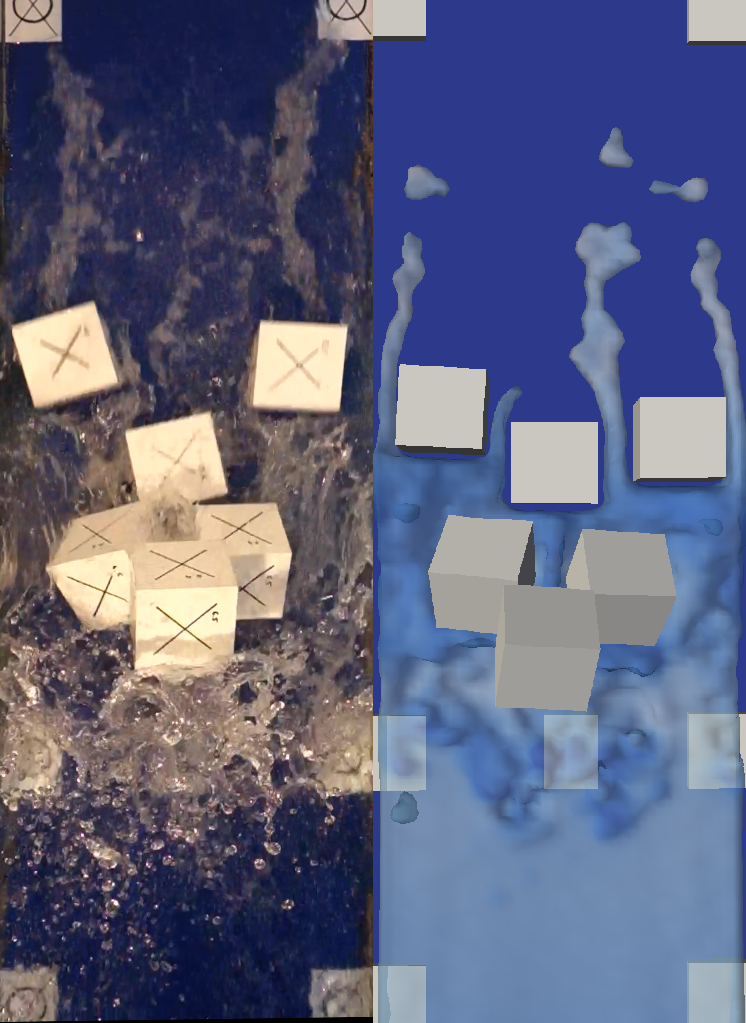
\includegraphics[width=0.35\linewidth]{Figures/5.Chapter/Fig_7b}	
	\caption{Configuration III. Experimental $vs$ numerical rendering of solution. Left $t=0.95s$, right $t=1.15s$.}
	\label{fig:figs_D2_IV} 
\end{figure}
%

The tracked cubes consist of the uppermost cube and the top left cube (observing from the perspective in Figure \ref{fig:lab_configs}). Figures \ref{fig:cube5_xy} and \ref{fig:cube5_z} show the results for the latter.
%
\begin{figure}[ht!]
	\centering 
	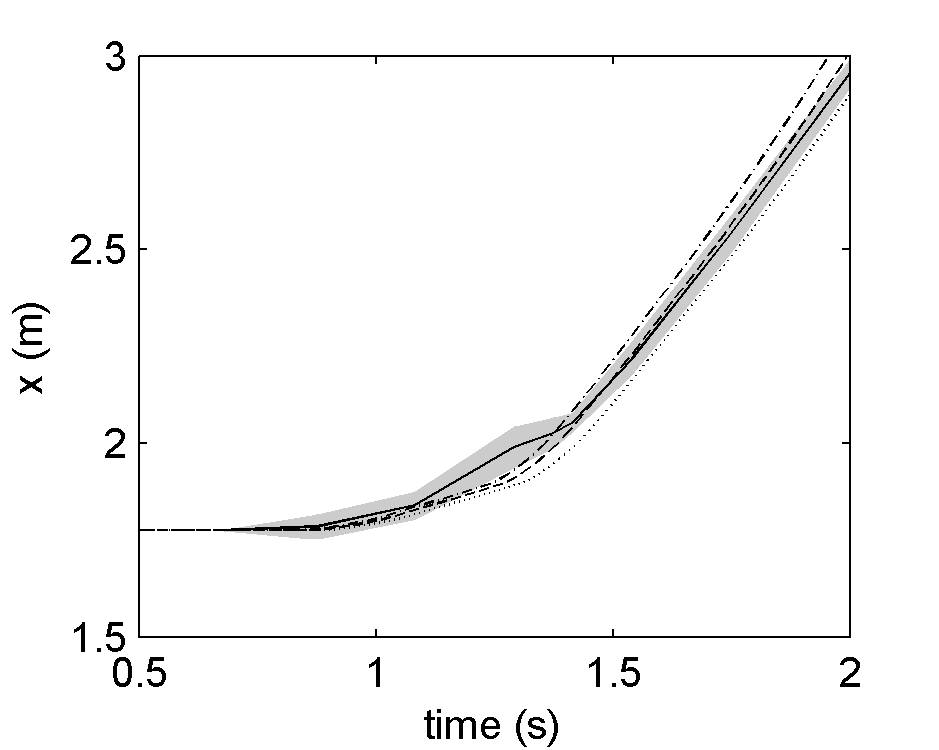
\includegraphics[width=0.45\linewidth]{Figures/5.Chapter/Fig_8a}
	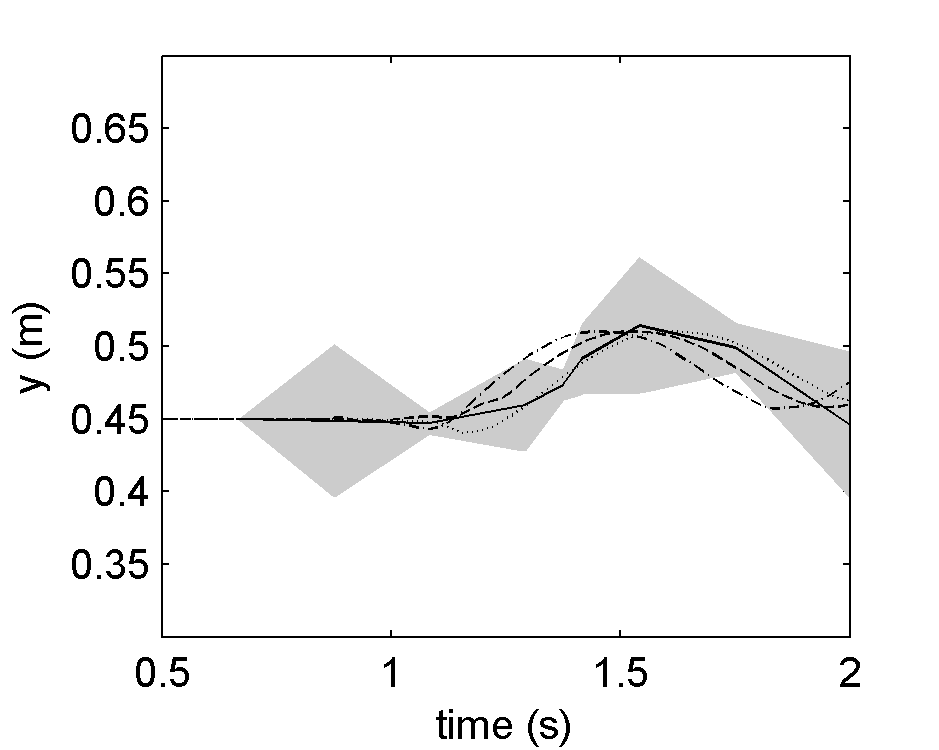
\includegraphics[width=0.45\linewidth]{Figures/5.Chapter/Fig_8b}
	\caption{Top left cube. Left - $x$ coordinates, Right - $y$ coordinates. Experimental (-), DualSPHysics $L/Dp=10 (- \cdot -)$, $L/Dp=15 (- -)$, $L/Dp=45 (\cdots)$.}
	\label{fig:cube5_xy} 
\end{figure}
%

The longitudinal component shows a very good agreement between experimental data and the numerical solution. Every stage of the motion along the $x$ direction seems to be correctly characterized. The cube has two contacts from the bottom cubes and one contact from the top cube, in an asymmetric configuration. This configuration, along with the fact that the cube is not centered in the flume, justifies analyzing the motion along the $y$ direction. One can see a deviation on $y$ position of around $30\%$ of the cube dimension. Such deviation seems to be recovered in the numerical solution with the correct magnitude, although out of phase in the lesser resolved cases. A good result seems to be achieved for the $L/Dp=45$ resolution.
%
\begin{figure}[ht!]
	\centering 

	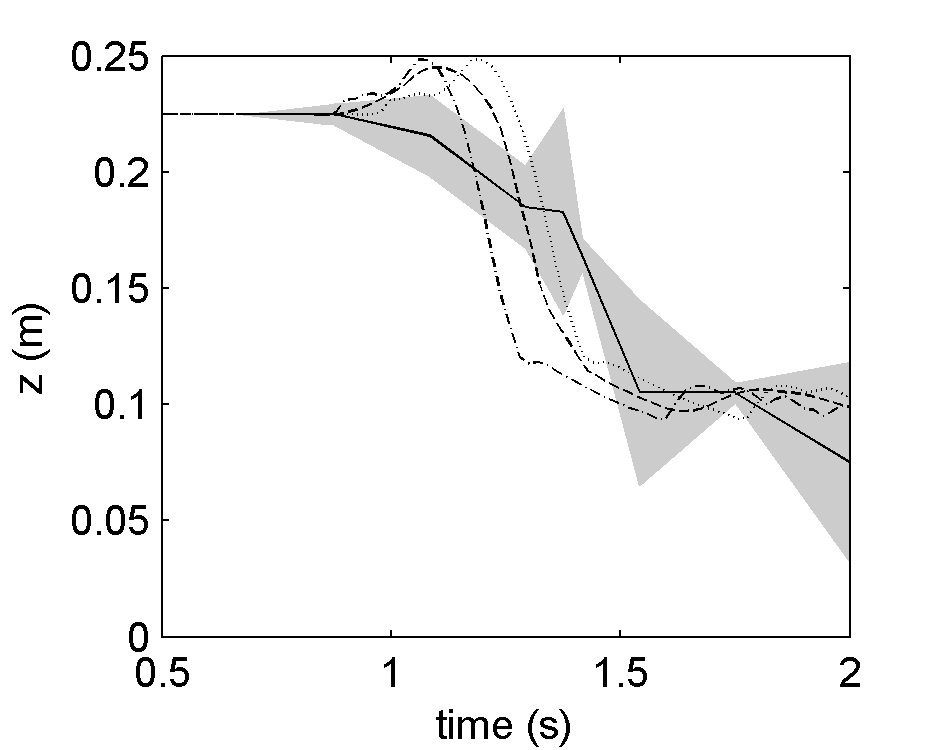
\includegraphics[width=0.45\linewidth]{Figures/5.Chapter/Fig_9}
	\caption{Top left cube. $z$ coordinates. Experimental (-), DualSPHysics $L/Dp=15 (- -)$, $L/Dp=10 (- \cdot -)$, $L/Dp=45 (\cdots)$.}
	\label{fig:cube5_z} 
\end{figure}
%
The vertical component of the motion is characterized is Figure \ref{fig:cube5_z}, showing a more sudden collapse on the numerical solution comparing to experimental data. An increase of height immediately prior to main motion, similarly to the behavior on Configuration II, is also observed.

The motion of the top cube is summarized in Figure \ref{fig:cube6}.
%
\begin{figure}[ht!]
	\centering 
	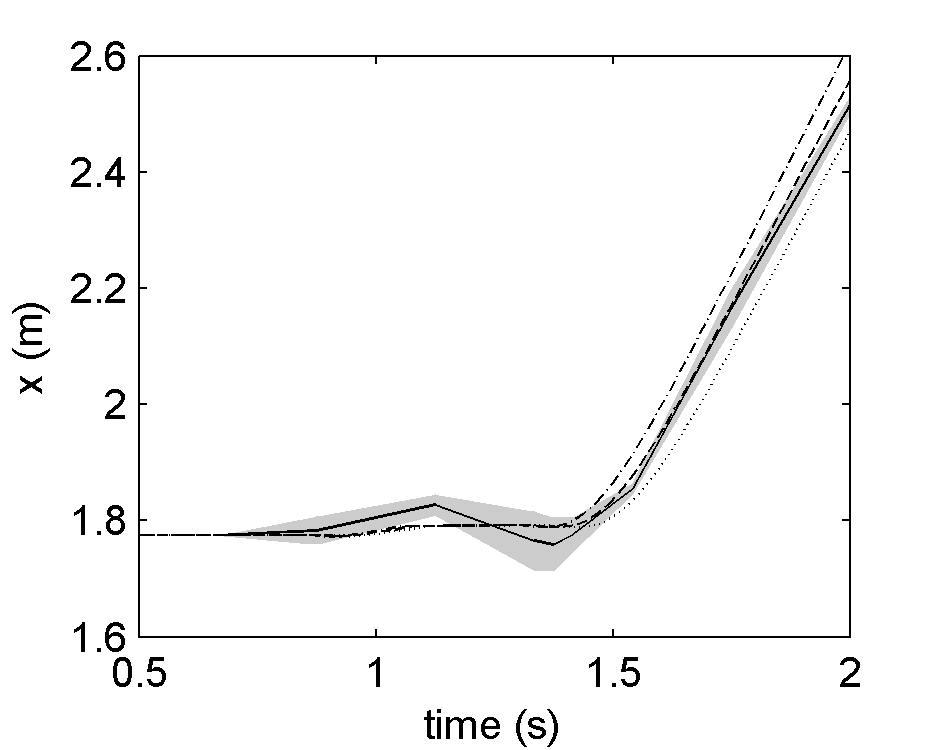
\includegraphics[width=0.45\linewidth]{Figures/5.Chapter/Fig_10a}
	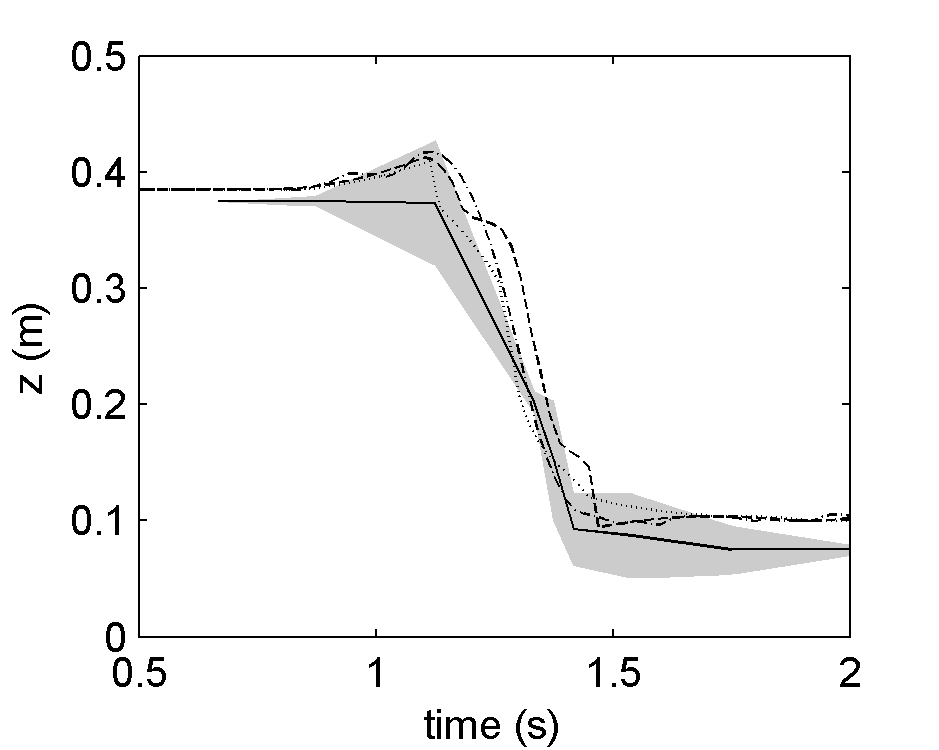
\includegraphics[width=0.45\linewidth]{Figures/5.Chapter/Fig_10b}
	\caption{Top cube. Left - X coordinates, Right - Z coordinates. Experimental (-), DualSPHysics $L/Dp=15 (- -)$, $L/Dp=10 (- \cdot -)$, $L/Dp=45 (\cdots)$.}
	\label{fig:cube6} 
\end{figure}
%
The results show the same trends as for other cubes. Both motions along the $x$ and $z$ directions show very good agreement, except for the defect along the $z$ axis at motion start. The effect seems to be independent from resolution, again indicating that the rigid body concept introduces an unavoidable small error for high velocity cases with multiple large bodies and multiple contacts.


\subsection{Flow field at impact locus}
\label{Subsect:PIV}

Reproducing Configuration I, a \ac{PIV} setup was used to recover the flow field once the front of the dam-break wave impacts the cube. The \ac{PIV} results may suffer with degraded signal since conditions are far from ideal: difficulty in homogeneous seeding due to transient nature, very unstable and discontinuous free surface, air bubbles are entrapped in the flow and may have a non-negligible velocity contribution and there is a large distance trough the flow from the laser sheet to the wall of the flume \citep{ferreira-2011}.

The \ac{PIV} system consisted of an 8-bit $1600\times1200$ px$^2$ CCD camera and a double-cavity Nd-YAG laser with pulse energy of $30$ mJ at wavelength of $532$ mn. The system was operated at $15$ Hz with a time delay of $1500\; \mu$s between frames. The seeding consisted of polyurethane particles with mean diameter of $60\; \mu$m in a range from $50$ to $70\; \mu$m and density of $1.31$ g/cm$^3$. At the available frequency, only one velocity field was captured, due to both movement of the object and free-surface deformation (initiation of splashes). Eight runs were completed and similar results were obtained each time, somewhat alleviating the concerns with the difficult test conditions. In order to facilitate the comparison of the flow field, \ac{SPH} data from a $L/Dp=45$ resolution was interpolated to the regular mesh produced at the output of the \ac{PIV} analysis, using the same \ac{SPH} kernel (Equation \eqref{eq:Kernel_wendeland}) as used to solve the system, with the same parameters. Figure \ref{fig:PIV_1} details the flow fields for experimental and numerical data.
%
\begin{figure}[ht!]
	\centering 
	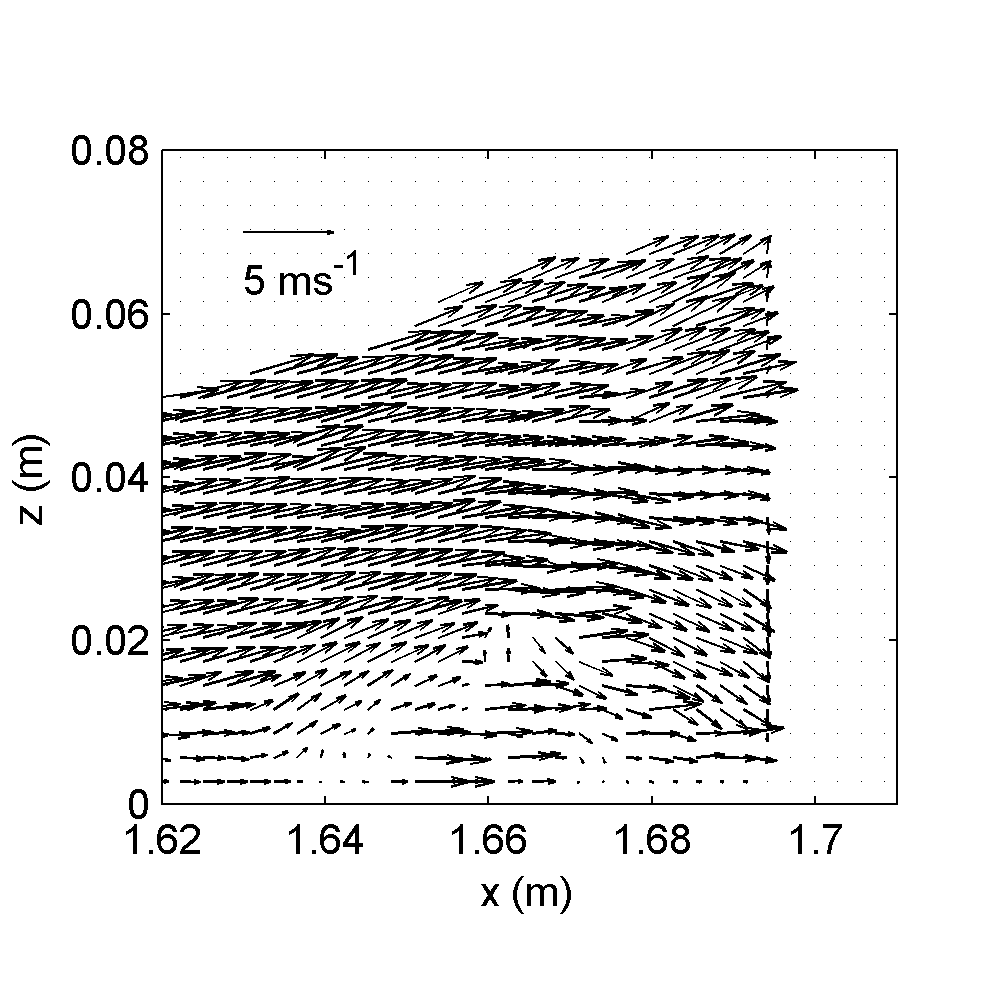
\includegraphics[width=0.45\linewidth]{Figures/5.Chapter/Fig_11a}
	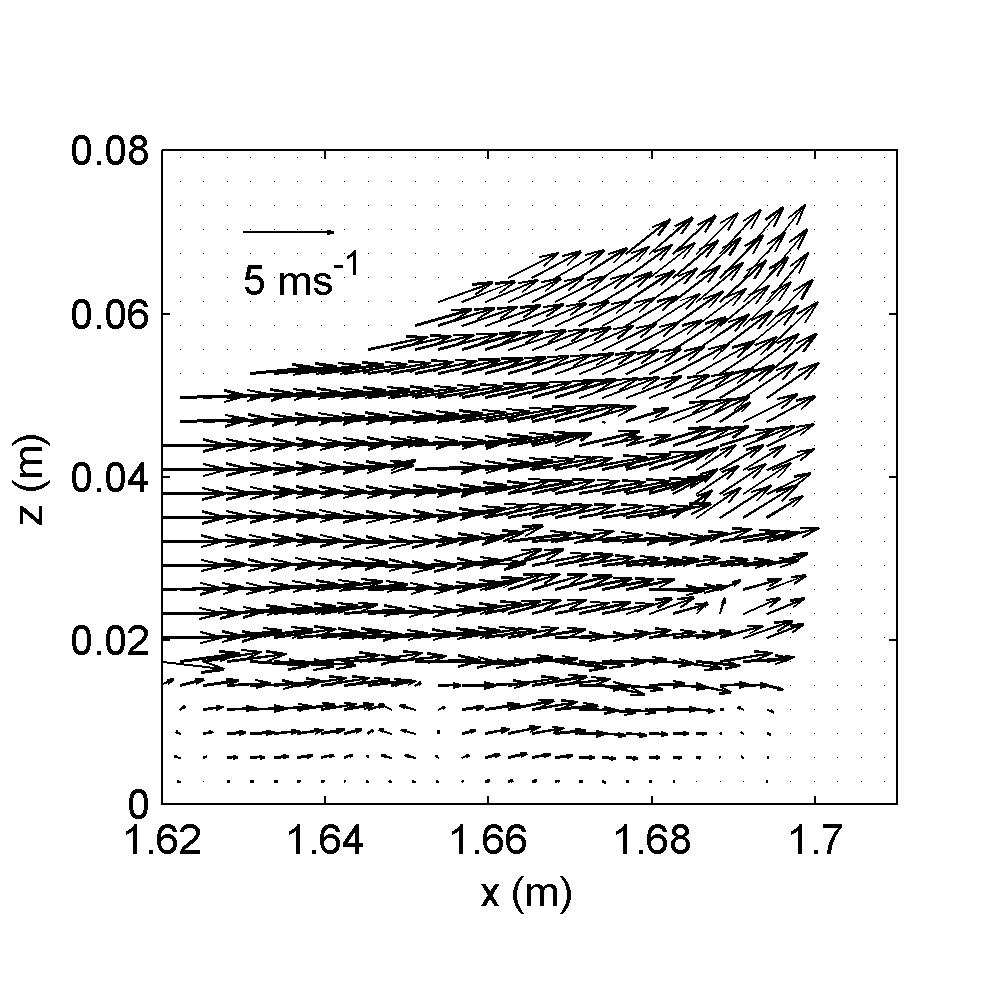
\includegraphics[width=0.45\linewidth]{Figures/5.Chapter/Fig_11b}
	\caption{Flow field at the impact locus, upstream of the cube in Configuration I. $t=0.88$ s. Left - Experimental data; Right - DualSPHysics $L/Dp=45$}
	\label{fig:PIV_1} 
\end{figure}
%

A separation point is detectable at mid-height of the flow depth in the experimental data, together with the formation of a recirculation structure near the bed. These structures are not fully formed, as their characteristic time scales are not compatible with the highly transient nature of the flow. The \ac{SPH} solution shows all  fundamental features of the flow: a stagnation point, a reduction of the velocity in the approach of the cube (indicating increasing pressure) and the influence of the bottom boundary. A less prominent stagnation point and a lack of a bottom recirculation pattern are visible. The velocity vectors are represented with the same scale, with maximum velocities around $3.7$ ms$^{-1}$, compatible with the Ritter solution \citep{stoker-1957} of 3.035 ms$^{-1}$ for the front of the wave.





